\documentclass[a4paper, 12pt, titlepage]{report}

\usepackage[english]{babel}
\usepackage{listings}
\usepackage{setspace}
\usepackage{color}
\usepackage{mathptmx}
\usepackage{titlesec}
\usepackage{lipsum}
\usepackage{graphicx}
\usepackage[dvipsnames]{xcolor}
\usepackage{hyperref}
\usepackage{amsmath}
\usepackage{pdfpages}
\usepackage{booktabs}
\usepackage{tabu}

\newcommand{\emptypage}{\newpage\shipout\null}
\newcommand{\autori}[1]{\textsc{\texttt{#1}}}
\lstset
{
	basicstyle=\scriptsize\ttfamily,keywordstyle=\color{OliveGreen},
	commentstyle=\color{blue},stringstyle=\color{red},showstringspaces=false,
   	breaklines=true,tabsize=4, frame=single, rulecolor=\color{black}
}

\newenvironment{dedication}
  {\clearpage           % we want a new page
   \thispagestyle{empty}% no header and footer
   \vspace*{\stretch{1}}% some space at the top 
   \itshape             % the text is in italics
   \raggedleft          % flush to the right margin
  }
  {\par % end the paragraph
   \vspace{\stretch{3}} % space at bottom is three times that at the top
   \clearpage           % finish off the page
  }
 
\renewcommand\labelitemii{--}
\renewcommand{\arraystretch}{1.5}

\begin{document} \sloppy \onehalfspacing
%\begin{frontespizio}
%	\begin{Preambolo*}
%	\renewcommand{\fonttitlefont}{\fontsize{20}{22}\bfseries}
%	\renewcommand{\frontinstitutionfont}{\fontsize{16}{17}\scshape}
%	\renewcommand{\frontdivisionfont}{\fontsize{14}{17}\bfseries}
%    	\renewcommand{\frontnamesfont}{\fontsize{14}{15}\bfseries}
%    	\renewcommand{\frontfixednamesfont}{\fontsize{14}{15}\bfseries}
%	\end{Preambolo*}
%
%\Istituzione{Università di Pisa}
%\Dipartimento{Ingegneria dell'Informazione}
%\Corso[Laurea Magistrale]{Computer Engineering}
%\Logo{img/stemma.jpg}
%\Titoletto{Tesi di Laurea Magistrale}
%\Titolo{High performance networking extensions for VirtualBox}
%\Sottotitolo{proca}
%\Candidato[468020]{Luca Carotenuto}
%\Relatore{Prof. Luigi Rizzo}
%\Relatore{Prof. Giuseppe Lettieri}
%\Annoaccademico{2015-2016}
%\end{frontespizio}
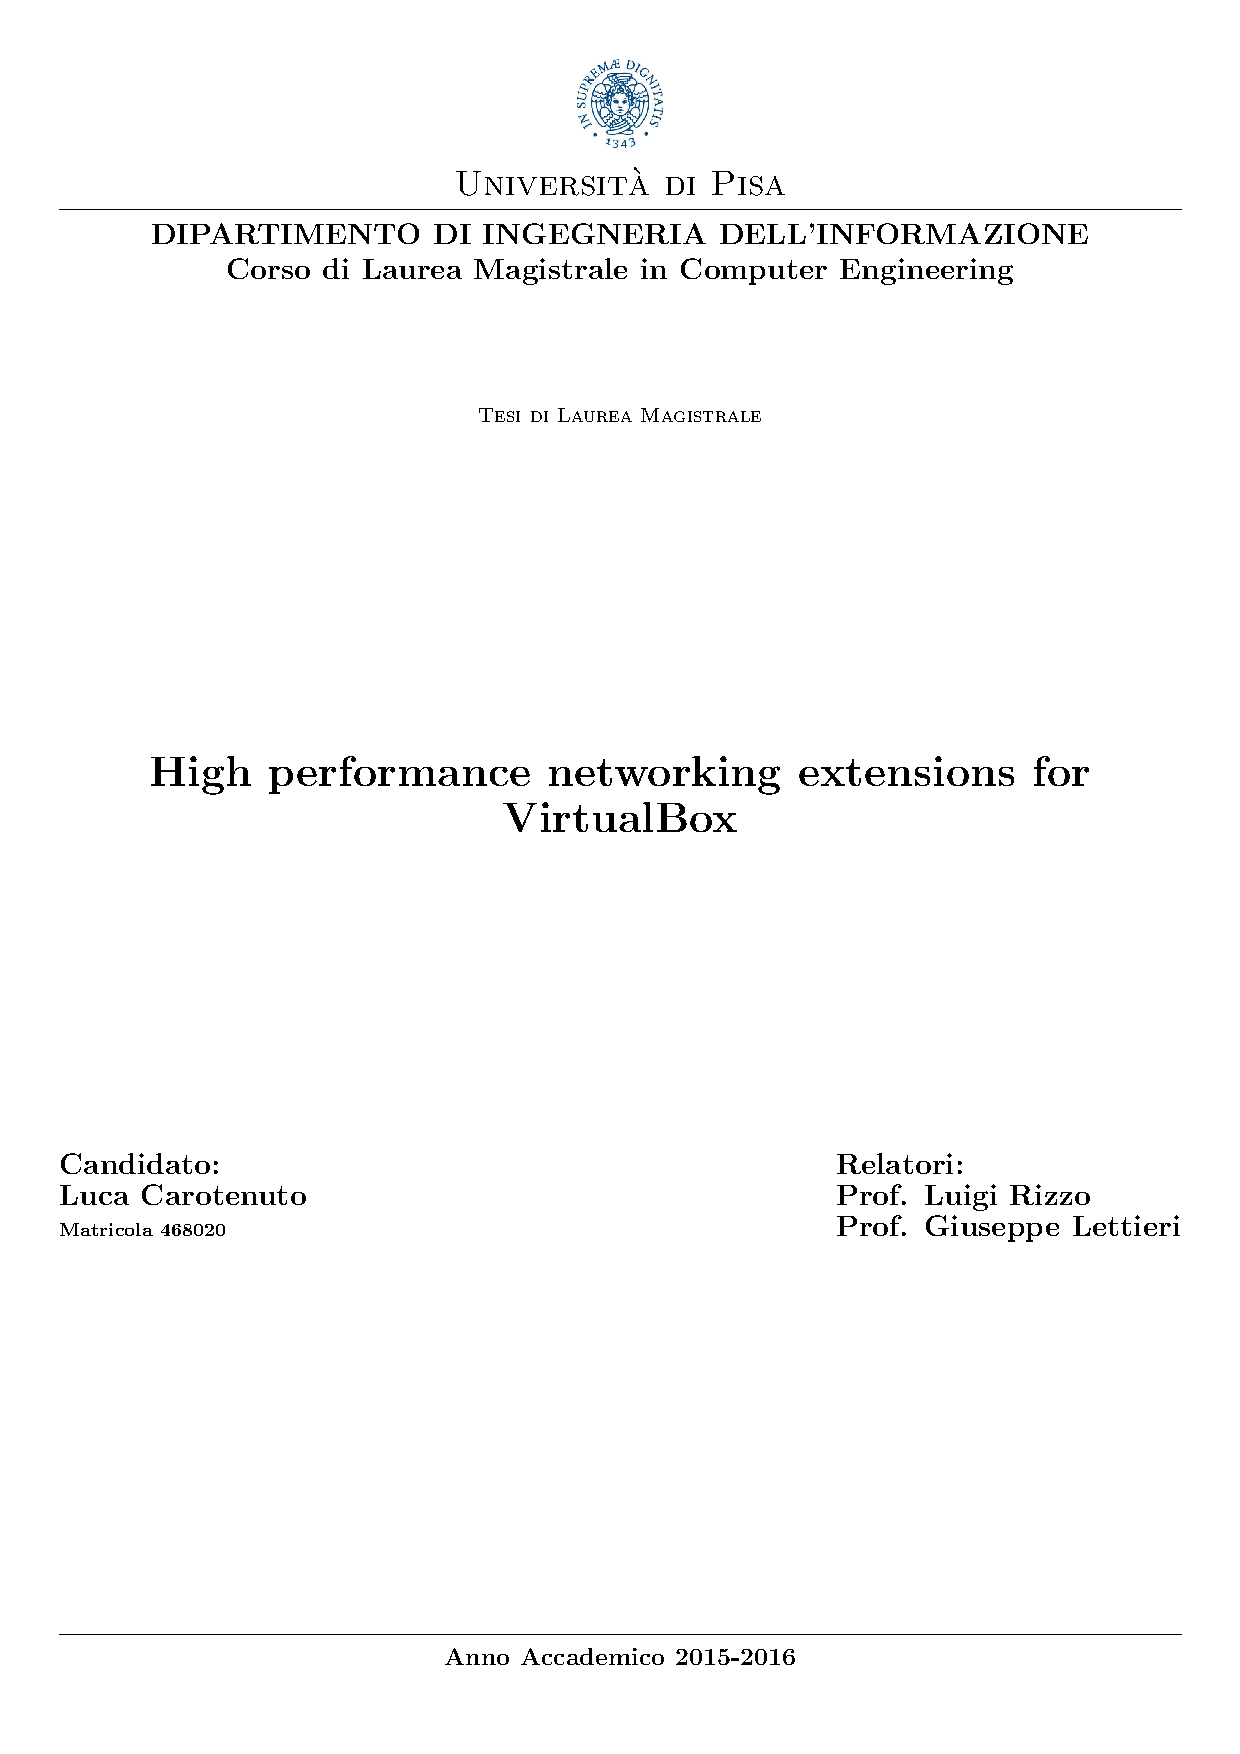
\includepdf{frontespizio.pdf}
\emptypage

\begin{dedication}
Alla mia famiglia,\\
a Erika,\\
ai miei amici.
\end{dedication}

\begin{abstract}
Virtual Machine systems are commonly used in several organizations providing network services, since those systems supply high reliability, security and availability. Therefore, network performance has become a critical issue to deal with, since Virtual Machine systems are widespread nowadays.
\\
\\
In this thesis we are going to present VirtualBox hypervisor, giving some details about its architecture and analyzing network performances of the existing solution. We then implement an extension that interfaces the hypervisor with netmap framework~\cite{netmap}, which provides fast packet I/O. Finally, we present some optimizations to an emulated network device (e1000 in our case), that considerably improve network performances.
\end{abstract}
\emptypage
\tableofcontents

\chapter{Introduction}

It is important to point out that the term \textit{Virtual Machine} may have multiple interpretations, so we must first specify which one of those meanings we are referring to.

When we talk about Virtual Machine (VM), we refer to a \textit{virtualized} computing environment running on top of a physical computing environment; as a result, we get one or more independent VMs, which may be different from the original one.\newline
Before proceeding, we introduce some terminology:
\begin{itemize}
\item \textit{Guest}: The VM.
\item \textit{Host}: The physical computing environment that \textit{hosts} one or more VMs.
\item \textit{Virtual Machine Monitor (VMM)}: The software part that provides support for virtualization. Also known as \textit{Hypervisor}.
\end{itemize}

The main reason that caused the spread of VMs is the abstraction levels that it introduces; this brings many benefits:
\begin{itemize}
\item \textit{Flexibility}: you can run programs compiled for a given Instruction Set Architecture (ISA) and/or a given Operating System (OS) on top of a computer that has a different ISA and/or different OS (e.g. you can test new software on different architectures without \textbf{having} one machine per architecture).
\item \textit{Protection}: each guest is \textbf{isolated}, which means that you can execute different applications on different VMs, so that if an application has a security issue, only the VM (or VMs) running that specific software will be exposed to it.
\item \textit{Resources usage}: one single physical machine may provide multiple services using the 100\% of the resources, instead of using many underutilized physical machines, thus reducing costs and saving energy.
\item \textit{Mobility}: replicating VMs to other locations is only a matter of copying/transmitting some files; this helps avoiding multiple setups since through a VM you can bring a functioning computing environment ready to use to the user.
\end{itemize}

As stated before, the term \textit{Virtual Machine} may have several meanings. A generic architecture of the "class" of VMs we will refer to (called \textit{Type 2 System Virtual Machines}), is shown in figure 1.1. In this case the VMM is a regular OS process, that runs in the host OS along with other processes. The VMM can access the physical resources through the OS services, which depend on the specific OS. We will not investigate other classes of Virtual Machines since this topic falls outside this work. 
\begin{figure}[!h]
	\centering
	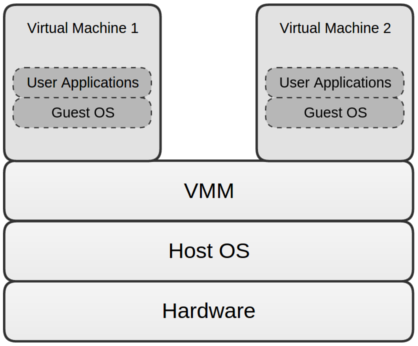
\includegraphics[scale=0.5]{img/vm_arch.png}
	\caption{Type 2 System Virtual Machine generic architecture}
\end{figure}

\section{Virtual Machine Implementation}
The basic idea behind VMs, is to \textit{emulate}, i.e. to execute code written for a certain environment, using another environment. In the following, we will briefly present the three basic techniques to implement emulation: interpretation, dynamic translation, hardware-based virtualization.
\subsection{Interpretation}
This is the naive emulation technique. The VMM has to perform in software what a physical CPU would have done in hardware: so it will be implemented as a loop, for each iteration, performs  the fetch, decode and execute phases of instruction execution.
\\
\\
Writing an interpreter for a modern ISA can be a very long and difficult process, even if it is conceptually simple; in fact, it is just a matter of reading an Instruction Set specification and implement all the possible instructions respecting the specifications.\\
However, the simplicity of this approach is responsible for its inefficiency; as a matter of fact, for each source instruction, the VMM has to execute many host instructions (e.g. 30-100) to perform in software all the necessary operations. The average \textit{translation ratio} is very high (e.g. 40).
\subsection{Dynamic translation} \label{subsec:dyn_tr}
This is a more sophisticated form of emulation. Rather than performing a "source-code-to-source-code" translation, the idea is to translate it into an equivalent binary code that can be executed directly on the host CPU.\\
This method amortizes the cost of interpretation, doing the fetch and decode phases only once or a few times. The code execution step of an instruction or a block of instructions is generated once (or a few times) and stored in a \textit{Code Cache}. After some time the code cache will contain the complete translation of the source program into the host ISA.\newline
As a result, the average translation ratio can be close to 1, giving an acceptable performance.
\\
\\
This technique is way more complicated than the previous one. In this case, several problems are present:
\begin{itemize}
\item \textit{code-discovery}: makes impossible to do static translation
\item \textit{code-location}: different address space of the guest and host systems
\item \textit{state mapping}: the way the VMM maps guest registers and the like to the host ones
\end{itemize}

It is interesting to notice that both interpretation and dynamic translation can make sense also in the case that guest and host have the same ISA; if this is the case, the translation is simplified since the code can be natively executed on the host machine, without performance losses.\\
However there are some cases where emulation in software my be necessary. As a typical example, memory accesses to the I/O space may need software emulation. In particular, if the guest wants to access a physical resource that is present on the host (e.g. a network adapter), the VMM cannot allow direct access to the device, because other processes could be accessing the same device at the same time, and, obviously, the host network driver and the guest network driver are not aware of each other. On the other hand, if the guest wants to access a virtual device (which does not exist on the host), the I/O instruction must be \textit{trapped}\footnote{Guest execution is interrupted and the VMM takes control.} in order to emulate the device behavior in software.

\subsection{Hardware-based virtualization} \label{subsec:hw_virt}
Due to the widespread use of VMs, extensions for virtualization were introduced by processor vendors. Thanks to these hardware assists, some of the problems affecting dynamic translation techniques have been overcome, and at the same time they have made it easier to execute guest code natively. Both AMD and Intel proposed their extensions for the x86 ISA, AMD-v (\cite{amd-v}) and VT-x (\cite{vt-x}) respectively.
\\
\\
With this new extension, the CPU can execute in two different modes: \textit{root mode} and \textit{VM mode} (or \textit{non-root mode}). The CPU can switch from root mode to VM mode through a so called \textit{VM entry} instruction, while can switch back to root mode through a so called \textit{VM exit} instruction. When in VM mode, the CPU can execute guest code in a controlled environment, i.e. the CPU cannot execute some safety-critical instructions (e.g. I/O instructions); when necessary, CPU performs a VM exit and runs host code (VMM or other processes). The switch operation between host world and guest world is similar to a context switch, since it involves the saving of the host state and loading the guest state (and vice versa). Although performed in hardware, these transitions between host and guest worlds are expensive in terms of performance, because software overhead, OS operations and userspace/kernelspace transitions are involved in the switching operations, but they are also necessary when dealing with I/O operations or interrupts. Hence, VM switches must be minimized in order to achieve good I/O performances.
\section{I/O Virtualization techniques}
Emulating a device means doing in software what the device would do in hardware. Thus, when a guest accesses an I/O device (e.g. writes to a device register), the VMM must take over and emulate all the operations associated with the specific I/O access.
\\
\\
In order to improve I/O virtualization techniques, three approaches have been defined:
\begin{itemize}
\item Hardware support in the devices (\textit{virtual functions} and IOMMU \cite{iommu}), so that a guest can directly access devices in a protected way and run at native speed.
\item Runtime optimizations in VMM. E.g. running short code involving multiple I/O instructions in interpreted mode saves some VM exits\footnote{See \cite{vmm_opt} for details.}.
\item Design \textit{virtual} device models in order to reduce expensive operations in device emulations (e.g. I/O accesses and interrupts). This approach is known as \textit{device paravirtualization} and produced some virtual device models, such as VirtIO (\cite{virtio}).
This requires synchronization and memory sharing between the guest and VMM in order to exchange information, while interrupts are used only for notification purposes. In that way it is easier to minimize the amount of VM exits.
\end{itemize}

\chapter{VirtualBox}
In this chapter we will present VirtualBox hypervisor, giving details about its features (section~\ref{sec:features}), its internal architecture (section~\ref{sec:architecture}), and how the behavior of e1000 device is emulated (section~\ref{sec:e1000_emu}).
\\
As host OS, we used Ubuntu 15.10 64-bit with kernel version 4.2.0. The guest OS is the same as the host one.

\section{VirtualBox features} \label{sec:features}
VirtualBox is a free, open source hypervisor, written entirely in C/C++. In particular, it is a cross-platform type 2 VMM, so it is able to run an arbitrary OS, regardless of the host OS, and it is implemented as a regular process in the host OS, therefore it can make use of all OS services. At the time of the writing, VirtualBox version number is 5.0.4, so we will refer to that version for Linux OS (since our host OS is Linux based).
\\
\\
Here is a brief outline of VirtualBox main features:
\begin{itemize}
\item \textbf{Portability.} VirtualBox runs on a large number of a 32-bit and 64-bit host operating systems. It can run VMs created on different hosts and/or with different virtualization software.
\item \textbf{Multiple virtualization interfaces.} VirtualBox provides three different virtualization interfaces
	\begin{itemize}
	\item \textit{Minimal}: Announces the presence of a virtualized environment.
	\item \textit{KVM}: Presents a Linux KVM hypervisor interface which is recognized by Linux kernels starting with version 2.6.25.
	\item \textit{Hyper-V}: Presents a Microsoft Hyper-V hypervisor interface which is recognized by Windows 7 and newer operating systems.
	\end{itemize}
We chose the KVM interface for tests and implementations.
\item \textbf{Multiple frontends}: A \textit{frontend} is a user interface that VirtualBox provides, such as:
	\begin{itemize}
	\item \textit{VBoxManage}: A textual interface that allows advanced settings for VMs.
	\item \textit{VirtualBox}: The default frontend, based on Qt~\cite{qt}.
	\item \textit{VBoxSDL}: An alternative frontend based on SDL~\cite{sdl}. This is useful for business use as well as testing  during development. The VMs then have to be controlled with VBoxManage.
	\item \textit{VBoxFB}: The "Framebuffer GUI", a GUI that sits directly on the Linux framebuffer. Not currently maintained.
	\end{itemize}
\item \textbf{No hardware virtualization required.} Even if hardware virtualization is fully supported, VirtualBox does not require the processor features such as Intel VT-x or AMD-V; in that way VirtualBox can be used also on old hardware which has not these features.
\item \textbf{Guest Additions.} VirtualBox Guest Additions are software package which can be installed \textit{inside} of supported guest systems to provide additional integration and communication with the host system (e.g. accelerated 3D graphics, automatic adjustment of video resolution and more).
\item \textbf{Great hardware support.} Among others, VirtualBox supports:
	\begin{itemize}
	\item \textbf{Guest multiprocessing (SMP).} VirtualBox can present up to 32 virtual CPUs to each virtual machine, regardless of how many CPU cores are physically present on the host.
	\item \textbf{USB device support}. VirtualBox implements a virtual USB controller that allows to connect arbitrary USB devices to VMs without having to install device-specific drivers on the host.
	\item \textbf{Hardware compatibility.} VirtualBox virtualizes a vast array of virtual devices. That includes IDE, SCSI and SATA hard disk controllers, several virtual network cards (including e1000) and so on.
	\item \textbf{Full ACPI support.} The Advanced Configuration and Power Interface (ACPI) is fully supported by VirtualBox.
	\end{itemize}
\item \textbf{Multigeneration branched snapshots.} VirtualBox can save arbitrary snapshots of the state of the VM. You can go back in time and revert the VM to any such snapshot and start an alternative VM configuration from there, effectively creating a whole snapshot tree.
\item \textbf{VM groups.} VirtualBox provides a groups feature that enables the user to organize and control VMs collectively, as well as individually.
\item \textbf{Clean and modular architecture.} VirtualBox has an extremely modular design with well-defined internal programming interfaces and clean separation of client and server code (i.e. code related to VMs and code related to the VMM, respectively).
\end{itemize}
\section{VirtualBox architecture} \label{sec:architecture}
In this section we will present the internal architecture of VirtualBox, giving details about its implementation that is necessary to understand in order to implement our optimizations.

\subsection{VirtualBox components} \label{subsec:components}
When the VirtualBox Graphical User Interface (GUI) is opened and at least a VM is started, three processes are running:
\begin{itemize}
\item \textit{VBoxSVC} is the VirtualBox service that always runs in background. This process is started automatically by the first client process~\footnote{i.e. a frontend. See section \ref{subsec:vbox ui} for more informations.} and exits a short time after the last client exits. The service is responsible for maintaining the state of all VMs. It is also called \textit{server} process
\item The GUI process. It communicates settings and state changes to \textit{VBoxSVC}. It is also called \textit{client} process
\item The hypervisor process.
\end{itemize}
When we launch VirtualBox (e.g. the VirtualBox GUI), the VBoxSVC component starts executing and initializes all the registered VMs. Then, when a VM is launched, before it starts executing, the client asks the server all settings the details, so that it can deliver these information to the starting VMM process. Finally, the hypervisor is able to execute the VM.
\\
In section~\ref{subsec:vm_settings} we will see these steps in details.

\subsection{VirtualBox kernel modules} \label{subsec:kern_modules}
VirtualBox provides different kernel modules that the user should add to the host kernel:
\begin{itemize}
\item \textit{vboxdrv}: The only mandatory module. This is needed by the VMM to gain control over the host system. It is used to manage the host/guest world switches and device emulations.
\item \textit{vboxnetadp}: "vboxnetadp" stands for "VirtualBox Network Adapter". It is needed to create a host networking interface (called \textit{vboxnet}); that interface (basically a virtual switch), is used to connect VMs to each other (and/or to the host). It is necessary when VirtualBox networking mode is set on \textbf{host-only} or \textbf{bridged} (these modes will be explained in section~\ref{subsec:net_modes}).
\item \textit{vboxnetflt}: "vboxnetflt" stands for "VirtualBox Network Filter". It is a kernel module that attaches to a real interface on the host and filters and injects packets. As for vboxnetadp, it is only necessary for host-only and bridged modes.
\item \textit{vboxpci}: This kernel module provides PCI card passthrough. This is used when the user wants to use a PCI device on the guest, even if the related driver is not available on the host.
\end{itemize}
\subsection{Software Virtualization}
As stated in section~\ref{sec:features}, VirtualBox fully supports hardware virtualization. However, since this is not a requirement, in the event that hardware virtualization is not present, VirtualBox makes use of a technique defined as \textit{Software virtualization}.
In order to understand the software virtualization technique, it is important to understand how CPUs provide a mechanism of protection at microcode level called \textit{Protection rings}.
\subsubsection{Privilege rings}
\begin{figure}[!h]
	\centering
	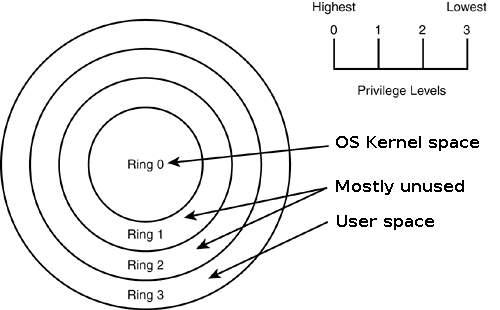
\includegraphics[scale=0.5]{img/rings.png}
	\caption{Protection rings}
\end{figure}
As shown in figure 2.1, there are four privilege levels or \textit{rings}, numbered from 0 to 3, with ring 0 (R0) being the most privileged and ring 3 (R3) being the least. The use of ring allows for system software to restrict task from accessing data or executing privileged instructions. In most environments, the OS and some device drivers run in R0 and applications run in ring 3~\cite{rings}.
\subsubsection{Software Virtualization}
In addition to the four privilege rings provided bu the hardware, we need to differentiate between \textit{host context} and \textit{guest context}.
\begin{itemize}
\item In \textit{host context}, everything is as if no VMM was active. This might be the active mode if another application on the host has been scheduled CPU time; in that case, there is a host R3 mode and a host R0 mode.
\item In \textit{guest context} a VM is active. So long as the guest code is running in ring 3, this is not much of a problem since a hypervisor can set up the page tables properly and run that code natively on the processor. The problems mostly lie in how to intercept what the guest's kernel does.
\end{itemize}
When starting a VM, through its R0 support kernel driver, VirtualBox has set up the host system so that it can run most of the guest code natively, but it inserted itself at the "bottom" of the picture. It can then assume control when needed, e.g. if a privileged instruction is executed, the guest \textit{traps}; VirtualBox may then handle this and either route a request to a virtual device or possibly delegate handling such things to the guest or host OS. In guest context, VirtualBox can therefore be in one of three states:
\begin{itemize}
\item Guest R3 code is run unmodified, at full speed, as much as possible. The number of faults will generally be low. This is also referred to as \textit{raw mode}, as the guest R3 code runs unmodified.
\item For guest code in R0, VirtualBox employs a trick: it actually reconfigures the guest so that its R0 code is run in \textbf{ring-1} (R1) instead. As a result, when guest R0 code (actually running in R1) such as a guest device driver attempts to write to an I/O register or execute a privileged instruction, the VirtualBox hypervisor in "real" R0 can take over.
\item The VMM can be active. Every time a fault occurs, VirtualBox looks at the offending instruction and can relegate it to a virtual device, the host OS, the guest OS, or run it in the \textbf{recompiler}.
\\
\\
In particular, the recompiler is used when guest code disables interrupts and VirtualBox cannot figure out when they will be switched back on. The recompiler is based on the dynamic translation technique (section~\ref{subsec:dyn_tr}).
\end{itemize}
Unfortunately this only works to a degree. Among others, the following situations require special handling:
\begin{enumerate}
\item Running R0 code in R1 causes a lot of additional instruction faults, as R1 is not allowed to execute any privileged instructions (of which guest's R0 contains plenty). With each of these faults, the VMM must step in and emulate the code to achieve the desired behavior. While this works, emulating thousands of these faults is very expensive and severely hurts the performance of the virtualized guest.
\item There are certain flaws in the implementation of R1 in the x86 architecture that were never fixed. Certain instructions that \textit{should} trap in R1 don't. If the guest is allowed to execute these, it will see the true state of the CPU, not the virtualized state.
\item A hypervisor typically needs to reserve some portion of the guest's address space for its own use. This is not entirely transparent to the guest OS and may cause clashes.
\item The SYSENTER instruction (used for system calls) executed by an application running in a guest OS always transitions to R0. But that is where the VMM runs, not the guest OS. In this case, the hypervisor must trap and emulate the instruction even when it is not desirable.
\item The CPU segment registers contain a "hidden" descriptor cache which is not software-accessible. The hypervisor cannot read, save or restore this state, but guest OS may use it.
\item Some resources must (and can) be trapped by the hypervisor, but the access is so frequent that this creates a significant performance overhead.
\end{enumerate}
To fix these performance and security issues, VirtualBox contains a \textit{Code Scanning and Analysis Manager} (CSAM), which disassembles guest code, and the \textit{Patch Manager} (PATM), which can replace it at runtime.
\\
\\
Before executing R0 code, CSAM scans it recursively to discover problematic instructions. PATM the performs \textit{in-situ} patching, i.e. it replaces the instruction with a jump to hypervisor memory where an integrated code generator has places a more suitable implementation. In reality, this is a very complex task as there are lots of odd situations to be discovered and handled correctly.
\\
\\
In addition, every time a fault occurs, VirtualBox analyzes the offending code to determine if it is possible to patch it in order to prevent it from causing more faults in the future. This approach works well in practice and dramatically improves software virtualization performance.
\subsection{Hardware virtualization}
As stated in section~\ref{subsec:hw_virt}, with Intel VT-x there are two distinct modes of CPU operation: root mode and non-root mode.
\begin{itemize}
\item In root mode, the CPU operates much like older generations of processors without VT-x support. There are four privilege rings, and the same instruction set is supported, with the addition of several virtualization specific instructions. Root mode is what a host operating system without virtualization uses, and it is also used by a hypervisor when virtualization is active.
\item In non-root mode, CPU operation is significantly different. There are still four privilege rings and the same instruction set, but a new structure called \textit{Virtual Machine Control Structure} (VMCS) now controls the CPU operation and determines how certain instructions behave. Non-root mode is where guest systems run.
\end{itemize}
The VMCS includes a guest and host state area which is saved/restored when switching between the two modes (\textit{VM entry} and \textit{VM exit}). Most importantly, the VMCS controls which guest operations will cause VM exits.
Thanks to the VMCS, a hypervisor can allow a guest to write certain bits in shadowed control registers,but not others. This enables efficient virtualization in cases where guests can be allowed to write control bits without disrupting the hypervisor, while preventing them from altering control bits over which the VMM needs to retain full control. The VMCS also provides control over interrupt delivery and exceptions.
\\
\\
Whenever an instruction or event causes a VM exit, the VMCS contains information about the exit reason. Thus the hypervisor can efficiently handle the condition without needing advanced techniques such as CSAM and PATM described above.
\\
\\
VT-x inherently avoids several of the problems which software virtualization faces. The guest has its own completely separate address space not shared with the hypervisor, which eliminates potential clashes. Additionally, guest OS kernel code runs at privilege R0 in non-root mode, obviating the problems by running R0 code at less privileged levels. Naturally, even at R0 in non-root mode, any I/O access by guest code still causes a VM exit, allowing for device emulation.
\\
\\
We restrict our work to the Hardware Virtualization solutions, because the optimizations we introduce are effective in limiting the amount of switches between root mode and non-root mode.
\subsection{Emulation Threads} \label{subsec:EMT}
When a VM is started, a user-defined number of SMP processors is assigned to the VM itself. Each CPU is emulated through a so called \textit{Emulation Thread} (EMT), so we have one EMT per SMP processor. An EMT is responsible of executing guest code, emulating devices and handle the transition between host world and guest world. 
\\
When using hardware virtualization (as we stated before, this is our case), an EMT continuously switches between root mode and VM mode (see section~\ref{subsec:hw_virt}).
\\
\\
Let us assume that the EMT is running guest code, e.g. an application. At some point, the application tries to execute an I/O operation, causing a SYSENTER instruction in the guest. Therefore, the CPU executing the EMT, switches from R3 to R0 (still in VM mode), in order to run the guest kernel code. At this point, the "true" I/O operation (such as a write operation in a register) produces a VM exit, so the CPU switches from VM mode to root mode. On a VM exit the EMT stops executing guest code and start executing VirtualBox code (in kernelspace), in order to handle the event that caused the VM exit itself. Handling a VM exit \textit{may} cause the EMT to execute userspace code in order to emulate a device, switching back to kernelspace after the device emulation (more on this in section~\ref{sec:e1000_emu}). After the event has been handled, the EMT executes a VM entry (i.e. CPU switches back to VM mode) and continues to run guest code from the point where it was interrupted.
\\
\\
\begin{figure}[!ht]
	\centering
	 	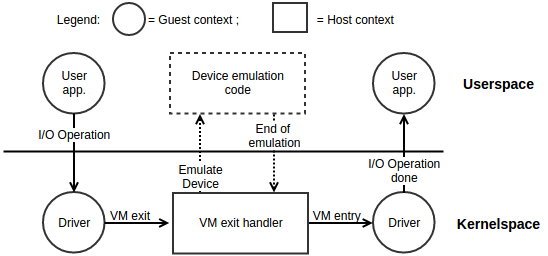
\includegraphics[scale=.75]{img/emt_flow.png}
	 	\caption{Example of EMT execution flow}
	 	\label{img:emt_flow}
\end{figure}
Figure~\ref{img:emt_flow} shows the situation described above.

\subsection{Networking modes} \label{subsec:net_modes}
For a VM it is fundamental to communicate to the outside world using the networking infrastructure, otherwise the VM becomes useless.
\\
Nevertheless, a VM is "just" a software entity, so it is not connected to any \textit{real} network. Therefore the VMM must provide some kind of virtualized network infrastructure, so that guest OS thinks its \textbf{virtual} network device is connected to a \textbf{physical} network and can then exchange packets with the outside.
\\
\\
VirtualBox provides several of these network infrastructures called \textit{Networking modes}; in that way a user can choose the most suitable way to connect her VM. Among the others, the main network modes provided by VirtualBox are the following:
\begin{itemize}
\item \textbf{Not attached} In this mode, VirtualBox reports to the guest that a network card is present, but there is no connection, as if no Ethernet cable was plugged into the card.
\item \textbf{Network Address Translation (NAT)} A VM with NAT enabled acts much like a real computer that connects to the Internet through a router. The "router", in this case, is the VirtualBox networking engine, which maps traffic from and to the VM transparently. In VirtualBox this router is placed between each VM and the host.
\\
The VM  receives its network address and configuration on the private network from a DHCP server integrated into VirtualBox. The IP address thus assigned to the VM is usually on a completely different network than the host.

\item \textbf{Bridged networking} With bridged networking, VirtualBox uses a device driver on the host system (\textit{vboxnetflt} kernel module) that filters data from the physical network adapter. That is why it is called "network filter" driver. This allows VirtualBox to intercept data from the physical network and inject data into it, effectively creating a new network interface in software. When a guest is using such a new software interface, it looks to the host system as though the guest were physically connected to the interface using a network cable: the host can send data to the guest through that interface and receive data from it. This means that the user can set up routing or bridging between the guest and the rest of the network.
\item \textbf{Internal networking} It is similar to bridged networking in that the VM can directly communicate with the outside world. However, the "outside world" is limited to other VMs on the same host which connect to the same internal network, which is identified simply by its name.
\\
Even though technically, everything that can be done using internal networking can also be done using bridged networking, there are security advantages with internal networking. In bridged mode, all traffic goes through a physical interface of the host system. It is therefore possible to attach a packet sniffer to the host interface and log all traffic that goes over it. If, for any reason, the user prefers two or more VMs on the same machine to communicate privately, hiding their data from both the host system and the user, bridged networking therefore is not an option.

\item \textbf{Host-only networking} Host-only networking can be thought as a hybrid between the bridged and internal networking modes: as with bridged networking, the virtual machines can talk to each other and the host as if they were connected through a physical Ethernet switch. Similarly, as with internal networking however, a physical networking interface need not to be present, and the virtual machines cannot talk to the world outside the host since they are not connected to a physical networking interface.
\\
Instead, when host-only networking is used, VirtualBox creates a new software interface on the host (using \textit{vboxnetadp} kernel module) which then appears next to the existing network interfaces. In other words, whereas with bridged networking an existing physical interface is used to attach virtual machines to, with host-only networking a new "loopback" interface is created on the host. And whereas internal networking the traffic between the VMs cannot be seen, the traffic on the "loopback" interface on the host can be intercepted.
\end{itemize}
NAT mode is not interesting with respect to our goals, since it is only intended to be a way the VM can easily access the Internet, and it is not intended to be an efficient networking mode. Similarly, we will not consider bridged networking mode, because optimizing the performance of a real network adapter is not the aim of this work. Instead, we will consider the host-only mode, since our goal is to optimize the communication performances between two VMs on the same host, or between a VM and the host (so also internal networking is not interesting for us), using the netmap framework.

\subsection{Network port and connector} \label{subsec:port_conn}
In order to implement a specific networking architecture, VirtualBox implementation includes an interface between the code that emulates the network adapter, and the code that provides access to the chosen networking mode. The reason is that the two subsystems are completely independent, and a user can easily combine every virtual network adapter with every networking mode.
\\
VirtualBox defines the network device emulation \textit{network port} and the networking mode \textit{network connector}.
\\
\\
Ports and connectors are two interfaces that communicate via a callback mechanism. In any way a code implements a port interface, it must have a reference (i.e. a pointer) to a connector, and vice versa.
\paragraph{Ports}
The methods~\footnote{The "pfn" prefix stands for "pointer to function". It is imposed by VirtualBox coding guidelines.} exported by ports (which are exposed to connectors) are the following:
\begin{itemize}
\item \texttt{pfnWaitReceiveAvail} Waits until there is space for receiving data. It also takes as argument the number of milliseconds to wait (timeout). If timeout parameter is 0, then it returns immediately. The return value specifies if there is space available to receive data, if timeout expired or if an error occurred.
\item \texttt{pfnReceive} When the connector receives data from the network, it calls this function on the port, so the latter can push data to the guest. This function takes the pointer to available data and the number of bytes in the buffer as arguments.
\item \texttt{pfnReceiveGso} The same as \texttt{pfnReceive}, but it has and additional argument regarding the \textit{segmentation offloading} context~\footnote{We are not going into details, since in our work we did not implement segmentation offloading.}.
\item \texttt{pfnXmitPending} This function is used to notify the port that can transmit pending packets (if any).
\end{itemize}
\paragraph{Connectors}
The methods exported by connectors (which are exposed to ports) are the following:
\begin{itemize}
\item \texttt{pfnBeginXmit} It is used by port to get a lock on the connector (only one port instance can transmit at a time).
\item \texttt{pfnAllocBuf} This asks the connector to provide the buffer that the port will fill with data. The size of that buffer is specified as an argument.
\item \texttt{pfnFreeBuf} Frees an unused buffer that has been requested by the port.
\item \texttt{pfnSendBuf} Sends data to the network. After the port filled the buffer (allocated by the connector) with data, it calls this function passing the filled buffer to the connector.
\end{itemize}
Moreover, both interfaces export two other (mandatory) methods: \texttt{pfnConstruct} (constructor) and \texttt{pfnDestruct} (destructor). The constructor is called when the VMM instantiates a port/connector, the destructor is called during the shutdown process.
\\
\\
\begin{figure}[!ht]
	\centering
	 	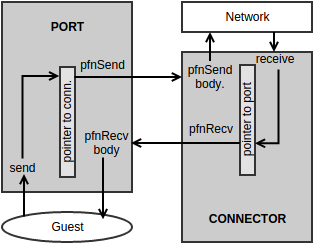
\includegraphics[scale=.75]{img/port_conn_if.png}
	 	\caption{Example of EMT execution flow}
	 	\label{img:port_conn_if}
\end{figure}In this way, when a port wants to send a frame to the network, it invokes the \texttt{pfnBeginXmit} function provided by the connector in order to gain lock access on the connector itself; then it calls \texttt{pfnAllocBuf} function to get a buffer where the port can store the frame and, finally, it invokes \texttt{pfnSendBuf} so that the connector can push the frame (passed as argument) to the network.
On the other direction, when the connector gets a frame from the network, it invokes the \texttt{pfnWaitReceiveAvail} to whether the port is able to receive data. If this is the case, it immediately calls \texttt{pfnReceive} so that the port can push the received frame (passed as argument) to the guest.
\\
A simplified version of the above interaction is depicted in figure~\ref{img:port_conn_if}, where only the \textit{send} and \textit{receive} functions are shown.

\section{The e1000 network adapter} \label{sec:e1000_adapter}
In this section we will outline of the functioning of an e1000 device. We will describe only those aspects that are relevant to our goals, in particular we are interested to the NIC \textit{datapath}. The complete specifications can be found at~\cite{e1000}
\\
\\
The datapath refers to the software interface that the OS uses in order to transmit and receive Ethernet frames. It involves just some registers and DMA-mapped memory.
\\
When the device driver wants to send an Ethernet frame through the adapter, it has to tell the adapter where the frame is stored in physical memory and how long it is. Once the device is aware of where the frame is stored, it can directly access the physical memory and send the frame on the wire. Similarly, when a frame arrives from the wire, the adapter has to store it in the physical memory. For this reason, it must know in advance where to store the frames, so the device driver must tell the adapter where it can store arrived frames. If it is not the case, the adapter will drop incoming frames.
\\
\\
As we can see, in order to achieve this information exchange, there must be a well-defined interface between the device driver and the adapter. This interface is known as a \textit{ring}. A ring is a circular \textbf{array} (i.e. a contiguous zone in memory) of \textit{descriptors} that are used to exchange  those information. A network device has at least two rings: one for transmission (\textit{TX ring}) and the other for reception (\textit{RX ring}). A network adapter can have multiple TX/RX rings, possibly with different priorities and/or policies, so that it permits traffic engineering.
\\
However, VirtualBox implementation of e1000 device, offers only one ring per direction. The number of descriptors per ring (i.e. the length of the array), can be chosen by the device driver. In e1000 this number must be a power of 2 and less than or equal to 4096.

\subsection{TX ring}
The TX ring is an array containing \textit{N} TX descriptors. Each descriptor is 16 bytes long and contains the physical address of the associated buffer, its length (i.e. the length of the stored frame) and some status flags. Among the others, it contains the \textit{Descriptor Done} flag (DD) and the \textit{End of OPeration} flag (EOP). The DD flag is set by the adapter to tell the device driver that the TX descriptor has been successfully processed. The EOP flag is used by the device driver to tell the adapter whether that TX descriptor contains a complete packet or only a part of it (e.g. because it does not fit in the buffer); so if a packet is spread among \textit{N} TX descriptors, the first \textit{N-1} descriptors will have the EOP flag set to 0, and the last one will have the flag set to 1.
\\
\\
Since the ring is stored in physical memory, the adapter must know its physical address. This information is stored in two registers: TDBAL (\textit{Transmit Descriptor Base Address Low}) and TDBAH (\textit{Transmit Descriptor Base Address High}). These are two 32-bit registers that, concatenated, form a 64-bit string of bits which is the physical base address of the ring.
\\
Since it is a producer/consumer system, a synchronization mechanism is required between the device driver and the adapter. This is achieved using two \textit{index registers}: the TDT register \textit{Transmit Descriptor Tail} and the TDH register \textit{Transmit Descriptor Head}. The value of these registers represent an \textit{array index} with respect to the TX ring.
\\
\\
At the beginning, TDT and TDH are initialized to their initial value (0) by the device driver. When the driver wants to send a new frame, it writes the physical address and the length of the frame in the descriptor pointed by TDT register, then it increments the TDT register itself (modulo number-of-descriptors).
\\
When the adapter recognizes that TDH and TDT are different, it understands that there are new frames to be sent on the wire, so it start processing the descriptors starting from the one pointed by TDH.
\\
For each new descriptor to process, the device:
\begin{enumerate}
\item Sends the new frame on the wire.
\item Writes the TX descriptor back in order to set the DD flag to 1.
\item Increments the TDH register circularly. 
\end{enumerate}

So the adapter can access the next descriptor to be processed with this formula:
$$Index = base + (TDH \times 16)$$
Where \textit{base} is the concatenation of TDBAH and TDBAL registers.
\\
\\
The \textbf{adapter} stop condition is \begin{math}TDH == TDT \end{math}, i.e. there are no more descriptors to process (TX ring empty).
\\
In order to prevent the index registers to wrap around, the device driver must never use the last free descriptor. So when the TDT is such that incrementing it circularly would cause \begin{math}TDH == TDT \end{math}, the driver must stop transmitting. This is the \textit{TX ring full} condition.
\\
Figure~\ref{img:tx_ring} shows the TX ring with its registers.
\begin{figure}[!h] 
	\centering
	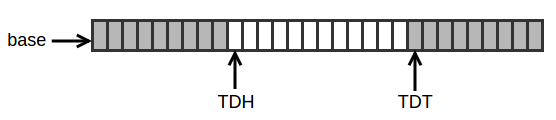
\includegraphics[scale=0.6]{img/tx_ring.png}
	\caption{TX ring with its registers. Free descriptors are the grey ones, while the pending descriptors are the white ones. \textit{base} is the concatenation of TDBAH and TDBAL registers.}
	\label{img:tx_ring}
\end{figure}

\subsection{RX ring}
The RX ring is an array of \textit{N} RX descriptors. Each RX descriptor is 16 bytes long and contains the physical address of the associated buffer, its length and some status flags. Among the others, it contains the DD flag and the EOP flag (just like a TX descriptor). The DD flag is used by the adapter to notify the device driver that a the RX descriptor contains new data to be processed. The EOP flag is used by the adapter to tell the device driver whether that RX descriptor contains a complete packet or only a part of it. So if a packet is spread over \textit{N} RX descriptors, the first \textit{N-1} will descriptors will have the EOP flag set to 0, while the last one will have the flag set to 1.
\\
\\
Just as for TX ring, the adapter must know the physical address of the RX ring. This address is stored in two registers: RDBAL (\textit{Receive Descriptor Base Address Low}) and RDBAH (\textit{Receive Descriptor Base Address High}). These are two 32-bit registers that, concatenated, form a 64-bit string of bits which is the physical base address of the RX ring.
\\
Here also, the synchronization between the adapter and the device driver is implemented through two index registers: RDT register (\textit{Receive Descriptor Tail}) and RDH (\textit{Receive Descriptor Head}).
\\
\\
At the beginning, the driver initializes RDH and RDT to their initial values (0). The adapter still does not know the physical address of any buffer where it can store frames, so it cannot store incoming frames. Therefore, the driver writes the physical address of a memory buffer into the RX descriptor pointed by RDT, and increment RDT circularly\footnote{It is useless to write the length field in the descriptor, since it will be modified by the adapter on reception.}. Now the device know that a new memory buffer is available, so it use it to store incoming frames. When $RDH \neq RDT$, the adapter knows that there are buffers available, so it can accept incoming frames.
\\
When a new frame is arrived from the wire, the adapter:
\begin{enumerate}
\item Fetches the RX descriptor pointed by the RDH register.
\item Copies the frame to the buffer pointed by the fetched RX descriptor.
\item Writes back the descriptor in order to set the length of the received frame and the DD bit (\textit{writeback}).
\item Increments RDH register circularly.
\item \textit{May} send an interrupt in order to tell the driver that a new frame is available to be delivered to the network stack\footnote{See section~\ref{subsec:rx_emulation}.}.
\end{enumerate}
So the adapter can access the next available RX descriptor with this formula:
$$Index = base + (RDH \times 16)$$
where \textit{base} is the concatenation of RDBAH and RDBAL registers.
\\
\\
The \textbf{adapter} stop condition is $RDH == RDT$, i.e. there is no available free descriptor where a frame can be stored.
\\
As for the TX ring, in order to prevent the array indexes to wrap around, the driver should never increment RDT if the increment would cause $RDT == RDH$. This is the full RX ring condition.
\\
Figure~\ref{img:rx_ring} shows the RX ring with its registers.
\begin{figure}[!h] 
	\centering
	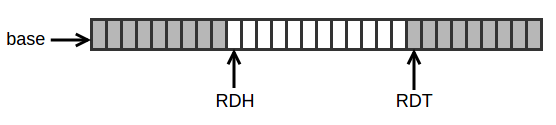
\includegraphics[scale=0.6]{img/rx_ring.png}
	\caption{RX ring with its registers. Filled descriptors are the grey ones, while the available descriptors are the white ones. \textit{base} is the concatenation of RDBAH and RDBAL registers.}
	\label{img:rx_ring}
\end{figure}

\subsection{e1000 interrupts} \label{subsec:e1000_interrupts}
The e1000 network adapter can generate interrupts for several reasons, but we are only interested in two of them:
\begin{itemize}
\item \textit{TX interrupts}: these interrupts are raised when the transmission of one or more frames completed. Each TX descriptor has a bit flag \textit{Report Status} (RS), that, if set, tells the adapter to raise an interrupt as soon as the associated frame is transmitted. Anyway, an interrupt is always sent when the adapter reaches the stop condition ($TDT == TDH$).
\\
The interrupt handler frees the descriptors that have been processed (DD flag set), and mark them as free (unset the DD flag).
\item \textit{RX interrupts}: these are raised whenever the adapter stores a new incoming frame in physical memory; in that way the device driver knows that a new frame has been received and it can be pushed to the kernel network stack.
\end{itemize}
When we are dealing with high packet rates, e.g. 1 Mpps, interrupt rate becomes a critical issue. In fact, interrupt routines have a fixed cost that must be paid before doing useful work, such as push the received frame to the network stack and let the receiver application to process it.
\\
At this rate, if each received packet raised a RX interrupt, the we would handle up to 1 million of interrupts per second, which would stall the machine. In that case, the CPU would spend almost all of its time in handling interrupts, and the receiver application could not do any useful work. This problem is known as the \textit{livelock} problem.
\\
\\
This problem can be solved if the device "skips" some RX interrupts, raising an interrupt every batch of received frames, e.g. 100 frames per batch, and not every single frame. In that way, the interrupt rate is 100 lower and the interrupt overhead is amortized over 100 frames. Anyway, the device must guarantee that a RX interrupt is raised after a period of time, even if the 100-frames batch is not completed, because the device cannot know when the next frame will arrive.
\\
These mechanisms are known as \textit{interrupt mitigation}. 
\\
The e1000 network adapter implements two interrupt mitigation mechanism, but since the older one is strongly discouraged by the Intel manual, we will consider only the most recent one.
\\
\\
The e1000 network adapter has a register, called \textit{Interrupt Throttling Register} (ITR), which controls the interrupt mitigation mechanism. If the driver sets this register to a value of $\delta$, the hardware ensures that $\delta$ is the minimum inter-interrupt interval, regardless of the interrupt type. In other words, whenever an event that requires an interrupt occurs, such as TX completion or RX completion, the device raises an interrupt as soon as possible, while meeting the ITR inter-interrupt delay constant.
\section{VirtualBox e1000 emulation}  \label{sec:e1000_emu}
The e1000 port is implemented in VirtualBox through three source files \footnote{These source files are located in src/VBox/Devices/Network/ in the VirtualBox project root directory.}: \textit{DevE1000.cpp}, which is the one we are interested in, \textit{DevE1000Phy.cpp} and \textit{DevEEPROM.cpp}. The first one contains all the "emulation logic" part, while the others implement only the internal physical emulation and the internal EEPROM respectively.
\\
The code is an implementation of the interfaces provided by VirtualBox. As mentioned in section~\ref{subsec:port_conn}, the first and last called method are the constructor (\texttt{pfnConstruct}) and the destructor (\texttt{pfnDestruct}) respectively. The main purpose of these functions is to register/deregister the new PCI Ethernet device with the rest of the emulator. In this way, it is possible to have multiple instances of the e1000 network device when launching VirtualBox.
\\
Furthermore, the code contains (in the first part of the file), a set of \textit{options} , implemented as \texttt{define} statements, that can be enabled/disabled before compiling (e.g. enable usage of caches, ITR register, and so on).
\\
\\
When registering a new PCI device, it is necessary to describe the I/O or MMIO regions that the device implements the device: this is done registering callback functions to to those regions, one for \textit{in} operations, on for \textit{out} operations.
\\
The e1000 emulation code registers a MMIO region and an I/O region, but the latter is not used. The MMIO region maps all the register the e1000 device implements.
\\
A statically defined mapping table is used to associate a couple of functions to each register, one for \textit{IN} operation, one for \textit{OUT} operation. In that way, one may associate a different read callback and a different write callback for each e1000 register. Is also possible to have the same callback function for multiple registers, or have no callbacks for some of them.
\\
In short, the emulation of a device is achieved with pre-registered callbacks.
\\
\\
Now we will see in details how the register callbacks are invoked.
\\
When an EMT is executing guest code, e.g. the e1000 device driver, it may try to access a MMIO location corresponding to an e1000 register. The accessing instruction causes a VM exit, so the EMT switches from the guest context to the host context. At this point, the VirtualBox driver analyzes the VM exit reason and understand that the VM exit was caused by an MMIO access. In our case, the callback registered with the e1000 MMIO is invoked. This callback uses the address to get the index of the accessed register and calls the read (write) handler specific for that register.
\\
After the callback returns, a VM entry is executed and the EMT resumes executing guest code.
\subsubsection{Event queues}
A register callback is invoked by the EMT (section~\ref{subsec:EMT}) while it is handling the VM exit event. So we are in R0 context. That said, writing a register may cause some side effects, therefore these side effects should be emulated. However, since it may take an amount of time that is, possibly, much longer than a simple register update, and also because it is unnecessary to execute that code in kernelspace, it is reasonable to execute the "side-effect" code in userspace.
\\
In order to achieve this, VirtualBox provides the so called \textit{Event queues}. As the name suggests, these are queues in which an \textit{event} can be posted. Each queue has a callback function that is associated to the queue itself.
\\
Every time the EMT finishes handling a VM exit it checks all the event queues before executing a VM entry. If an event is found, the EMT removes that event from the queue and switches from R0 context to R3 context, so that it can start executing the callback associated to that queue. 
\\
When the callback returns, the EMT switches back to the kernelspace and continues scanning all event queues. Finally, when there are no more pending events, it executes a VM entry and resumes executing guest code.

\subsection{TX emulation}
The TX execution path is performed in by the EMT thread. As described in section ~\ref{sec:e1000_adapter}, when the device driver wants to notify the hardware that a new TX frame is ready to be processed, it writes to the TDT register. This causes a VM exit to occur, so the EMT passes from guest context to host context.
\\
Writing to the TDT register causes the adapter to transmit one or more frames, so the transmission handling must be done in userspace. So the write callback for the TDT register, aside from updating the register value, posts an event to an event queue (\textit{TxQueue}); in this way the EMT, before switching back to the guest world, executes the transmission of frames in userspace.
\\
The callback associated with the event queue simply calls the \texttt{e1kXmitPending} function. The way this function is implemented is regulated from the \texttt{E1K\_WITH\_TXD\_CACHE} define.
\\
\\ 
When TX descriptors cache is disabled, the \texttt{e1kXmitPending} function:
\begin{enumerate}
\item \textit{Tries to acquire the lock} It calls the \texttt{pfnBeginXmit} function provided by the connector, where it \textbf{tries} to acquire the lock on the connector itself. This is a so called \textit{trylock} function, because if the lock is busy, the thread does not block waiting for the lock to be acquired. Instead, the function returns a \textit{busy} value. This is necessary because the thread trying to get the lock is the EMT, so it \textbf{must never} block, since it is in charge of emulating all the system.
If the trylock succeeds, then go to the next step, otherwise the function returns without doing any transmission.
\item \textit{Loads the current descriptor} If there are available descriptors ($TDT \neq TDH$), then it reads the TX descriptor pointed by TDH register from the guest physical memory.
\item \textit{Allocates buffer} The port asks the \textit{connector} to allocate the buffer where it can store the frame, which is pointed by the loaded TX descriptor. The information about the length of the frame is contained in the TX descriptor itself.
\item \textit{Writes back the descriptor} It writes the descriptor back into the guest physical memory, setting the DD bit to 1.
\item \textit{Copies the frame} It reads the physical address pointed by the current descriptor (where the frame is stored) and copies it into the buffer provided by the connector.
\item \textit{Possibly Transmits frame} If the packet is complete, i.e. EOP flag of TX descriptor is set to 1, then it calls the \texttt{pfnSendBuf} provided by the connector, passing the previously allocated buffer as an argument.
\item \textit{Updates register} It circularly increments the TDH register.
\item \textit{Possibly raises an interrupt} If at least one complete packet has been sent, it \textit{may} raise an interrupt to notify the guest that one or more frames have been sent (see section~\ref{subsec:e1000_interrupts}). If there are other descriptors available ($TDT \neq TDH$), then go back to step 2.
\item \textit{Releases the lock} After all operations, it releases the lock acquired at step 1 calling the \texttt{pfnEndXmit} provided by the connector.
\end{enumerate}
We can see that for each available descriptor, the EMT must read the guest physical memory in order to get the current TX descriptor. This introduces an high overhead, particularly when the number of available descriptors is much higher than 1.
\\
\\
The reading overhead can be amortized using a local TX descriptor cache. This can be done enabling the related option (\texttt{define E1K\_WITH\_TXD\_CACHE}).
\\
When the cache is enabled, the \texttt{e1kXmitPending} function behaves much like the same as before, except for the step 2. Previously, we had one TX descriptor per read. Now, instead, the EMT \textbf{tries} to load all the available TX descriptors in one single physical read (two reads in case the tail wrapped around the end of the TX descriptor ring). However, it may happen that only a fraction of the available descriptors is loaded, e.g. the cache is almost full. In that case, after the partial loading, the fetched descriptors are processed (like the previous case), the frames are sent and the cache is flushed, so that other available descriptors can be loaded.
\\
In that way, the cost of the readings is amortized over the number of fetched descriptors.

\subsection{RX emulation} \label{subsec:rx_emulation}
This time the RX execution path is not performed by the EMT, but it is performed by another thread. The reason is that the EMT is in charge of the entire emulation process, so it must never do blocking operations, so it cannot wait for incoming frames from the network.
\\
The thread in charge of receive frames is dependent on the used connector: in fact the frames flow from the network to the connector, and the latter sends them to the port (see section~\ref{subsec:port_conn}, figure~\ref{img:port_conn_if}).
\\
From now on, we will refer to this thread as \textit{recv thread}.
\\
\\
When one or more frames from the network, the recv thread stores them in a buffer (that is dependent from the connector implementation). Then it first calls the port callback \texttt{pfnWaitReceiveAvail} to check if the port is able to receive at least one frame. If that callback returns successfully, the thread calls the \texttt{pfnReceive} callback, passing the buffer with the available data.
\\
\\
The e1000 port implements the \texttt{pfnReceive} method with \texttt{e1kR3NetworkDown\_Receive} function, which takes the buffer and the size of the available data in the buffer as arguments.
\\
As in the TX case, the behavior (i.e. the implementation) is controlled by the \texttt{E1K\_WITH\_RXD\_CACHE} define.
\\
\\
When RX descriptor cache is disabled, this function:
\begin{enumerate}
\item \textit{Filters the packet} It determines if the packet is to be delivered to the upper layer. The decision is based on:
	\begin{itemize}
	\item Length: if the packet length is greater than the maximum supported size (16384 bytes) or if long~\footnote{Packet greater than 1522 bytes.} packet reception is disabled~\footnote{For further information, see~\cite{e1000}.}, then drop the packet.
	\item VLAN tag: if the filter does not find a match for the VLAN tag, then drop the packet.
	\item Exact Unicast/Multicast: if the packet destination address exactly matches the address (either unicast or multicast address), then deliver the packet, otherwise drop it.
	\item Promiscuous Unicast/Multicast: if the adapter is set in promiscuous mode~\footnote{The adapter accepts packets even if they are not addressed to it}, then deliver the packet, otherwise drop it.
	\item Broadcast: if the packet destination address is broadcast, deliver it.
	\end{itemize}
\item \textit{Pads the packet} If the received packet is too short (less than 60 bytes), the packet is padded with zeroes.
\item \textit{Loads the RX descriptor} If there is at least one available RX descriptor ($RDT \neq RDH$), then it loads the RX descriptor pointed by RDH register from the guest physical memory.
\item \textit{Fills the buffer} After loading the RX descriptor, it writes the (possibly padded) packet into the buffer pointed by the loaded RX descriptor. If the packet does not fit the buffer, the EOP flag of the RX descriptor is set to 0, otherwise the flag is set to 1.
\item \textit{Writes back the RX descriptor} After the RX descriptor has been filled with data, it sets the DD bit to 1 and writes back the RX descriptor in memory.
\item \textit{Updates register} It circularly increments the RDH register.
\item \textit{Possibly raises an interrupt} If at least one complete packet is successfully delivered, it \textit{may} raise an interrupt to notify the guest that one or more frames have been received (see section~\ref{subsec:e1000_interrupts}). If there is still data to be processed (e.g. a packet is not completely stored), go back to step 3.
\end{enumerate}
When the reception is completed (i.e. the \texttt{pfnReceive} function returns), the recv thread goes back to sleep waiting for new incoming packets.
\\
\\
Just as in the TX case, we can see that for each available descriptor, the recv thread must read the guest physical memory to get the current RX descriptor. Therefore we have an high overhead, in particular when we are dealing with large incoming packets.
\\
\\
This overhead can be amortized using a local RX descriptor cache, that can be enabled through the related option (\texttt{define E1K\_WITH\_RXD\_CACHE}). When the cache is enabled, the \texttt{e1kR3NetworkDown\_Receive} function behaves much like before, except for what concerns the loading of RX descriptors. In the previous case, we had one single RX descriptor per read. Now the recv thread, instead of loading the descriptor in memory, looks at the local cache: if the cache is empty, it \textit{prefetches} a number of RX descriptors, which is the minimum between the cache size and the number of available RX descriptors in memory, with a single memory read (two reads in case the tail wrapped around the end of the RX ring). If the cache is not empty, it uses the first available RX descriptor in cache.
\\
After the RX descriptor is processed and written back, the related position in cache is cleaned.
\\
\\
It is important to point out that the physical \textbf{guest} memory is different from the physical \textbf{host} memory. Therefore, all the accesses to the guest physical memory (such as TX/RX descriptor loads) require an \textit{address translation}, that introduces additional overhead. The way it can be obviated will be described in section~\ref{subsec:memmap}.

\chapter{Implementation of netmap support}
In chapter 2 we described the VirtualBox architecture, its implementation and the interfaces it provides. In this chapter we will implement an extension to VirtualBox that provides fast packet I/O. This is achieved by interfacing VirtualBox with the netmap framework~\cite{netmap}.
\\
\\
As described in section~\ref{subsec:port_conn}, VirtualBox includes two interfaces in order to implement the networking infrastructure: \textit{ports} and \textit{connectors}. Our goal is to create a new connector that implements the interfaces a VirtualBox port to a VALE switch~\cite{vale} provided by the netmap framework.
\\
Our netmap connector will be implemented through one single source file: \textit{DrvNetmap.cpp}\footnote{This source file will be located in src/VBox/Devices/Network/ in the VirtualBox project root directory. The \textit{Drv} prefix in the filename is due to the VirtualBox coding guidelines.}.

\section{Integration with VirtualBox} \label{sec:integration}
Before going into details of our implementation, we must first "integrate" our work in VirtualBox system. It basically involves the VirtualBox build process, the user interface, so that a user can choose netmap as connector for his system, and the VMs configuration mechanism, in order to set/save/load the new configuration parameters needed by netmap.

\subsection{Building VirtualBox}
The VirtualBox build process is performed through two steps: the configuration and the compilation.

\subsubsection{Configuration}
Before starting the compilation process, we must run the script \textit{configure}\footnote{Located in the root directory of VirtualBox project.}, in order to check if the system meets the requirements, e.g. the presence of needed libraries, and to let the user to specify some custom options (e.g. the \texttt{--disable-docs} option prevents the compilation of documentation files). Therefore, we added the "\texttt{--with-netmap=}\textit{dir}" option to that script, so that the user can specify the absolute path~\footnote{It is requested the path to the subdirectory \textit{sys} of netmap source tree, e.g. \texttt{--with-netmap=/path/to/netmap/sys/}.} of netmap libraries in the system.
\\
The effect of the new option is to set an environment variable that the Makefile will check, so that it knows whether to include or not our \textit{DrvNetmap.cpp} source file in the compilation process, and the netmap headers in the list of directories to be searched for header files\footnote{\texttt{-I} option of GNU C compiler.}.

\subsubsection{Compilation}
As mentioned before, the Makefile will check a netmap-related environment variable that can be enabled through the configuration process. VirtualBox has one \textit{virtual} Makefile, that is actually splitted in many files (more than two hundreds). Those files are organized in a hierarchical manner: there is one Makefile for each level of the source tree. Therefore, the more we go deeper in the source tree, the more specific the present Makefile is for that subtree.
\\
Since our new file will be placed in the network devices directory, we will modify the devices-related Makefile, located in \textit{src/VBox/Devices/} directory.

\subsection{The VirtualBox User Interface} \label{subsec:vbox ui}
As stated in section~\ref{sec:features}, VirtualBox offers multiple frontends as user interfaces. We need to extend those interfaces so that a user can choose netmap as connector.
\\
We focused on the \textit{VirtualBox} frontend (the default one), and \textit{VBoxManage} frontend, since \textit{VBoxSDL} only launches a VM, but the related configuration is done through VBoxManage.

\subsubsection{VirtualBox frontend}
This is the default frontend. It offers a user-friendly Graphical User Interface (GUI). The related source files are located in \textit{src/VBox/Frontends/VirtualBox/src}. Since we are interested in the networking part, we will focus on it.
\\
\begin{figure}[!ht] 
	\centering
	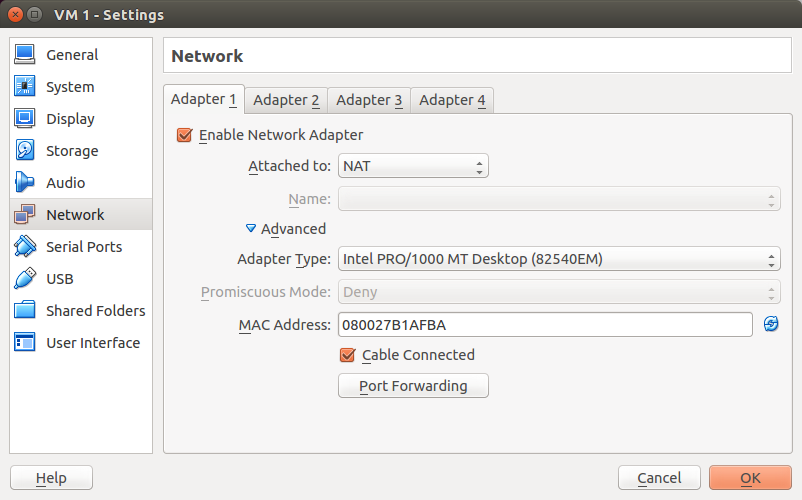
\includegraphics[width=\textwidth]{img/net_settings.png}
	\caption{Sample of VirtualBox network settings tab. In this case the adapter is an e1000 device, that is bridged to the host interface \textit{eth2}.}
	\label{img:vbox_net_settings}
\end{figure}As shown in figure~\ref{img:vbox_net_settings}, VirtualBox frontend allows to specify network settings for each VM independently and, for each VM, to specify up to 4 different network adapters. For each adapter, the following options are available:
\begin{itemize}
\item \textit{Enable flag} If checked, the network adapter is enabled in the Guest.
\item \textit{Attached to} This drop down menu specifies the connector the adapter will be attached to. See section~\ref{subsec:net_modes}.
\item \textit{Name} It is used in some networking modes. E.g. the bridged mode needs to know which physical interface will be bridged with the emulated interface.
\item \textit{Adapter Type} Here we can select the preferred emulated adapter (such as an e1000 device).
\item \textit{Promiscuous mode} It is used to set/unset the promiscuous mode on the adapter.
\item \textit{MAC Address} The MAC address of the emulated interface.
\item \textit{Cable Connected} If enabled, the adapter will be (virtually) connected to the connector.
\item \textit{Port Forwarding} Only in NAT mode.
\end{itemize}
Our goal is to extend this interface so that a user can choose netmap as preferred connector. What we have to do is to include netmap in the "\textit{Attached to}" drop down menu, then add an additional text box where some netmap parameters can be specified by the user.
\\
To achieve this, we modified some source files that define this frontend. They are located in \textit{src/VBox/Frontends/VirtualBox/src/settings/machine}. In that way, we added netmap as an item of the drop down menu and we used the \textit{name} field as a textbox to specify to which netmap port the adapter will be attached to (e.g. a vale switch).\\\\\begin{figure}[t] 
	\centering
	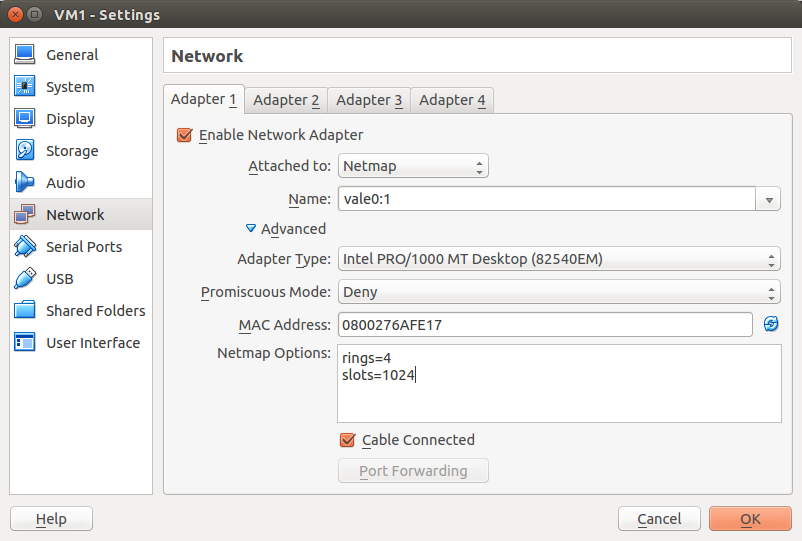
\includegraphics[width=\textwidth]{img/netmap_settings.png}
	\caption{The extended VirtualBox network settings interface. It uses the port 1 of the vale0 netmap virtual switch (vale0:1) and specifies 4 netmap rings per direction, having 1024 slots each.}
	\label{img:netmap_settings}
\end{figure}Moreover, we modified the \textit{UIMachineSettingsNetwork.ui} file; this file, which is used by Qt designer tool, describes all the GUI elements in XML (e.g. textboxes, flags, etc). Therefore, we added in the GUI a textbox where the user can specify some netmap parameters, such as the number of netmap rings and the related number of netmap slots~\footnote{For further information, refer to~\cite{netmap}.}.
\\
Figure \ref{img:netmap_settings} shows the result of our modifications.

\subsubsection{VBoxManage frontend}
VBoxManage is a Command Line Interface (CLI) that allows the user to completely control VirtualBox from the command line. VBoxManage supports all the features that the GUI gives the user access to, but it supports a lot more than that. VBoxManage must always be used with a specific \textit{subcommand}, such as \textit{createvm, modifyvm, controlvm} and others~\footnote{For a full list of available commands and their functions, refer to~\cite[chapter~8]{vbox}.}.
\\
The \textit{modifyvm} subcommand allows the user to specify many options for a specific VM, included the networking ones. So, what we have to do is to modify this command so that it supports netmap connector, netmap device name and netmap options. To achieve this we must modify the related source files in order to extend the command.
\\
\\
The source files are located in \textit{src/VBox/Frontends/VBoxManage/} and there is a file for each subcommand. Therefore, since we are interested in the modifyvm command, we modified the \textit{VBoxManageModifyVM.cpp}.
\\
We extended the \texttt{--nic} option, which specifies the connector, so that it recognizes netmap as an argument. Then, we added two more options to the subcommand:
\begin{itemize}
\item \texttt{--nicnetmapdev} It specifies the netmap device the adapter will be attached to (just like the \textit{name} field in the GUI.
\item \texttt{--nicnetmapoption} It specifies the netmap parameters (number of netmap rings and so on).
\end{itemize}
Furthermore, we modified the file \textit{VBoxManageHelp.cpp}, that is the implementation of the \texttt{help} command, so that the above netmap options and extensions are shown to the user.

\subsection{VirtualBox VM settings} \label{subsec:vm_settings}
In section~\ref{subsec:vbox ui} we discussed about how the user can interact with VirtualBox in order to tell it how to configure a VM. In the following, we will show how VirtualBox uses these information to actually configure a VM.

\subsubsection{XML settings file}
In VirtualBox, each VM has one directory where all files of that machine are stored; in particular, there is an XML file that describes the VM and all its settings.
\\
The settings file contains all those information that a user can specify for that specific VM, in particular the networking ones, using either the GUI frontend or the VBoxManage frontend. Therefore, when a user sets some options for a VM, e.g. specifies a certain connector, the information is stored in the related settings file.
\\
\\
Since we modified the user interface so that it recognizes netmap, now we have to tell VirtualBox how to \textit{parse} the information coming from the UI.
\\
This is achieved by modifying the file \textit{/src/VBox/Main/xml/Settings.cpp}, that contains functions which manage the XML settings file. Here we extended the functions that read (write) the settings file so that they are able to return (store) the netmap-related information.

\subsubsection{VirtualBox internal configuration}
As mentioned in section~\ref{subsec:components}, when a VM is started, we have three processes: \textit{VBoxSVC} (the server), the frontend process (the client) and the VMM process (that runs the VM).
\\
The VBoxSVC code is splitted in several source files located in \textit{src/VBox/Main/src-server/} directory, due to its modularity, but the only components we are interested in are:
\begin{itemize}
\item \textit{VirtualBoxImpl.cpp} It is the main component, the "core" of the server process. It is able to communicate with all other components.
\item \textit{MachineImpl.cpp} The \textit{Machine} component. It is an abstraction of a VM. It pares the XML settings file.
\item \textit{NetworkAdapterImpl.cpp} The \textit{NetworkAdapter} component. It is the component that manages the networking settings.
\end{itemize}
The client code is also splitted in several source files located in \textit{src/VBox/Main/src-client/} directory, but the only part we are interested in is the \textit{ConsoleImpl2.cpp} one, since it initializes the VM components.
\\
\\
From now on we will focus only on the handling of the networking settings, since it is the only relevant part for our purposes.
\\
\\
When we launch VirtualBox (e.g. the GUI frontend), the server process starts executing and initializes all the registered VMs through an \textit{init} function. For each VM, that function, asks the machine component to load the (networking) settings for that specific VM from the related XML settings file. After reading the XML file, the machine component gives the NetworkAdapter component the settings information, so that it can store them in its internal structure.
\\
\\
When we launch a VM, before the VM starts executing, the client asks the server process (VBoxSVC) all the (networking) settings details. The information request is then handled by the NetworkAdapter component, that returns the needed information.
\\
The client then: 
\begin{enumerate}
\item Discriminates which is the port/connector type using the information retrieved from the server.
\item Initializes two configuration data structures that will contain all the networking details returned by the server.
\item Delivers to the VMM the information about which port/connector has been chosen by the user and the related data structure. In that way the VMM knows which port/connector has to instantiate among all registered~\footnote{See section~\ref{subsec:registration}.} ones.
\end{enumerate} 
So, in the end, when the port and the connector will be instantiated by the VMM, i.e. the VMM will call the respective constructors, the related configuration data structures will be passed to the constructors as arguments.
\\
\\
In order to integrate netmap-related options, we had to extend both server and client codes. In particular we modified the \textit{VirtualBoxImpl.cpp}, \textit{NetworkAdapterImpl.cpp} and \textit{ConsoleImpl2.cpp} source files.

\paragraph{Server code} 
In \textit{NetworkAdapterImpl.cpp} source file we added some statements used to get/set the new netmap options from/in the internal data structure (e.g. when the machine component initializes this network component). Moreover we added two new methods, a \textit{getter} and a \textit{setter}, that are exposed to the main component so that it can get/set the netmap options.
\\
In \textit{VirtualBoxImpl.cpp} source file we added the \textit{getter} method (which calls the new getter function in the NetworkAdapter component) that is exposed to the client so that it can retrieve the new netmap-related information.

\paragraph{Client code} 
In \textit{ConsoleImpl2.cpp} source file there is a code part that discriminates all the registered connector types. Therefore, we extended that part by adding a possible case in which a netmap connector has been specified. Our code gets the netmap settings\footnote{These settings are the netmap device name (e.g. vale0:1) and, possibly, the netmap options.} from the server, puts them in the configuration data structure and deliver these information to the VMM.

\subsection{Connector registration} \label{subsec:registration}
Compiling our new source file and configuring it through a frontend is not sufficient to make the VMM aware of the new connector. In fact, VirtualBox separates the \textbf{configuration} from the \textbf{registration} of a port/connector.
\\
\\
In the initialization phase the VMM registers all connectors by calling the global function \texttt{VBoxDriverRegister} defined in \textit{VBoxDD.cpp} source file, located in \textit{src/VBox/Devices/build} directory. This, in turn, for each available connector in VirtualBox (not necessarily configured), calls the registration function that takes the pointer to the \textit{Driver Registration Record}.
\\
The driver registration record is a data structure containing some information about the connector itself that each connector has to statically allocate. These information are basically the name of the connector, the connector class (in our case is a network class connector) and a list of callbacks, such as the constructor and the destructor callbacks. Since a connector is identified by its name, it must be unique among all connectors. Furthermore, this registration record is useful to the VMM on startup. For these reasons, the structure must have a global scope.
\\
\\
As explained in section~\ref{subsec:vm_settings}, during the startup of a VM, a client tells the VMM which connector has to instantiate and delivers it the related settings information.
\\
The VMM scans the list of registered connectors looking for a connector having a name that matches with the one given by the client. If a match is found, then the VMM instantiates the matching connector and calls the constructor using the pointer specified in its driver registration record.
\\
\\
It is clear that if we do not register our new connector, the VMM will not be able to instantiate it and, therefore, our code will never be executed.
\\
In order to register our connector, we simply added a couple of lines of code in \textit{VBoxDD.cpp} source file, that call the register function passing the netmap driver registration record as argument. This registration record is contained in our new source file \textit{DrvNetmap.cpp}, which implementation will be described in the next section.

\section{Connector implementation} \label{sec:implementation}
In section~\ref{sec:integration} we discussed how we extended VirtualBox so that it is now "aware" of netmap. In the following, we will show our implementation of connector code.

\subsection{Internal data structures} \label{subsec:structs}
As we mentioned in section~\ref{subsec:registration} we need the driver registration record in order to register our new connector. The most relevant fields in the registration record are:
\begin{itemize}
\item Connector name, which identifies it among all other connectors. In our case is "Netmap"
\item The class of the connector. It could be an audio connector, a block connector and so on. In our case it is a network connector.
\item Pointer to the constructor function (\texttt{pfnConstruct}). It points to our constructor function, which name is \texttt{drvNetmapConstruct}.
\item Pointer to the destructor function (\texttt{pfnDestruct}). It points to our destructor function, which name is \texttt{drvNetmapDestruct}.
\end{itemize}
Once our driver registration record is ready, we must instance the data structure that will implement (and extend) the network connector interface. The data structure contains:
\begin{itemize}
\item \texttt{INetworkUp} The connector interface data structure. This contains the pointers to the functions~\footnote{See section~\ref{subsec:port_conn}, paragraph \textbf{Connectors}.} that we will implement.
\item \texttt{pIAboveNet} A pointer to the port interface we are attached to. With this, we can invoke the callbacks~\footnote{See section~\ref{subsec:port_conn}, paragraph \textbf{Ports}.} exposed to the port.
\item \texttt{pDrvIns} The pointer to a structure used to retrieve the actual instance of the connector.
\item \texttt{pszDeviceName} A string containing the name of the netmap device (e.g. vale0:1).
\item \texttt{pNetmapDesc} The netmap descriptor data structure.
\item \texttt{pTxSgBuf} A scatter/gather structure (S/G structure). This contains the buffer in which the port writes the frame it wants to transmit and some related information.
\item \texttt{pIOThread} A pointer to the asynchronous I/O thread.
\item \texttt{hPipeRead} The read end of a control pipe. It is read only by the asynchronous I/O thread.
\item \texttt{hPipeWrite, hPipeRead} The write end of a control pipe. It is written by the EMT and by the VMM. 
\item \texttt{XmitLock} The transmit lock that must be acquired by the port.
%\item \texttt{fNoAvailableSpace} A flag used to check if there is enough space for transmission.
\end{itemize}

\subsection{Connector initialization} \label{subsec:netmap_init}
Since the constructor is the first called function, this will be our starting point. The function that implements the \texttt{pfnConstruct} interface is called \texttt{drvNetmapConstruct}. Its purpose is to initialize our internal data structure (see section~\ref{subsec:structs}). It takes the pointer to the structure of the instance of the connector and the pointer to the configuration data structure.
\\
The basic steps this function performs are:
\begin{enumerate}
\item \textit{Initialization of the connector interface} For each callback exposed to the port, it assigns the related implementation.
\item \textit{Parsing of the configuration} It parses the configuration parameters given by the user~\footnote{See section~\ref{subsec:vm_settings}.}. For example, if the netmap device name is missing (which is mandatory), then the constructor returns an error shutting down the VM. The same happens if a user specifies some parameters not supported by netmap.
\item \textit{Opening of netmap descriptor} It calls the \texttt{nm\_open} function\footnote{Provided by the netmap user API.} using the user-specified parameters, if any, otherwise it uses the default ones. Opening a netmap descriptor involves the allocation of the netmap rings and, the netmap slots and, therefore, the buffer associated with each slot. Once that these buffer are allocated, their memory is never freed until the netmap descriptor is closed.
\item \textit{Initialization of lock and pipe} It initializes the transmit lock structure and the control pipe.
\item \textit{Thread creation} It instantiates the asynchronous thread, which has to handle the asynchronous I/O operations. The thread is instantiated with a function exposed by the VMM. In that way, the VMM takes care of suspending, resuming and destroying the thread as the VM state changes. In particular, this function takes two functions as arguments: the body of the thread, and the wakeup callback. This is called on the VMM on a VM state change~\footnote{See section~\ref{subsec:netmap_recv}.}. 
\end{enumerate}
When the VM is shutdown, the VMM destroys all the connectors instances by calling the destructor (\texttt{pfnDestroy}) function on each connector. Our implementation is a function called \texttt{drvNetmapDestruct}, and it performs almost all the operations done by the constructor backwards. In particular, it closes the pipe, deletes the lock and closes the netmap descriptor.
\\
The asynchronous thread destruction is performed internally by the VMM.
\subsection{Send side} \label{subsec:netmap_send}
In this section we explain the implementation of the operations related to the send side. In the following we will show, step by step, what happens on the connector side when a port wants to send a frame~\footnote{This implementation is not e1000 dependent, since it must work with any port.}.
\begin{enumerate}
\item \texttt{drvNetmapNetworkUp\_BeginXmit} Implements: \texttt{pfnBeginXmit}. When a port wants to transmit, the first thing it has to do is to acquire the lock on the connector. This function performs a trylock operation~\footnote{The transmitting thread is the EMT, so it must never block.} on the connector internal lock (\texttt{XmitLock}). If this operation is successful, the thread has exclusive access to the connector, so that there cannot be races.
\item \texttt{drvNetmapNetworkUp\_AllocBuf} Implements: \texttt{pfnAllocBuf}. After the lock acquisition, the port asks the connector to allocate the data structure, the S/G buffer structure, where it will store the packet. Since we are using netmap, the buffers associated with the netmap slots are allocated on the initialization phase (constructor), so there is no need to dynamically allocate/free memory. Therefore, we keep a statically allocated S/G structure (\texttt{pTxSgBuf}) which parameters will be configured on each \texttt{pfnAllocBuf} call. In particular, the buffer pointer in \texttt{pTxSgBuf} will point to the available netmap slot buffer. The function returns a pointer to \texttt{pTxSgBuf}. This allows to save the overhead caused by memory allocation/deallocation.
\\
However, it may happen that the netmap TX rings are full, so there is no space available for transmission. If this is the case, we try to flush  any potential pending slots by calling a \textit{TX\_SYNC} on the netmap File Descriptor (FD) through the \texttt{ioctl} system call. If this has no effect~\footnote{E.g. we are transmitting on a netmap pipe and there is no one reading on the other end.}, we %set the \texttt{fNoAvailableSpace} flag, 
write one byte with value \texttt{1} on the write end of the control pipe (the effects will be explained in~\ref{subsec:netmap_recv}) and return.
\item \texttt{drvNetmapNetworkUp\_FreeBuf} Implements: \texttt{pfnFreeBuf}. This is called by the port when it wants to free the previously allocated buffer~\footnote{E.g. at the end of transmission, or if an error occurred during some phase.}. In our case, since the buffer points to the netmap slot buffer, this function will simply reset the fields of \texttt{pTxSgBuf} instead of actually freeing the memory.
\item \texttt{drvNetmapNetworkUp\_SendBuf} Implements: \texttt{pfnSendBuf}. After the port has successfully filled the buffer, it calls this callback on the connector. This function increments the indexes of the netmap ring and performs a \textit{TX\_SYNC} on the netmap FD.
\item \texttt{drvNetmapNetworkUp\_EndXmit} Implements: \texttt{pfnEndXmit}. This simply releases the transmit lock on the connector.
\end{enumerate}
There are two additional callback functions: \texttt{pfnSetPromiscuousMode} and \texttt{pfnNotifyLinkChanged}. These two functions are not useful for our purposes, but since it is mandatory that a connector implements all the exported methods, we just implemented these two callbacks with two stub functions.

\subsection{Receive side} \label{subsec:netmap_recv}
In this section we will explain the implementation of the operations related to the receive side. In the following we will show, step by step, what happens on the connector side when a frame is received from the "outside world"~\footnote{This implementation is not e1000 dependent, since it has to work with any port}.
\\
\\
In section~\ref{subsec:netmap_init} we stated that the constructor initializes the thread that will handle the asynchronous I/O operations. We called this thread \textit{NETMAP thread}. Mostly, the thread is in charge of handling the incoming frames.
\\
\\
The reception must be necessarily handled by a dedicated thread, and not the EMT, because it has to \textbf{wait} for incoming packets. In our case, the thread must do a \texttt{poll} system call on the netmap FD~\footnote{For further information refer to~\cite{netmap}.}, which is a blocking operation.
\\
The NETMAP thread body is implemented by \texttt{drvNetmapAsynchIOThread} function, while its wakeup callback is implemented by \texttt{drvNetmapAsynchIOWakeup}. The wakeup callback writes one byte with value \texttt{0} to the write end of the pipe (\texttt{hPipeWrite}) and returns. The body of the thread, instead, performs two different phases: the initialization and the loop.
\\
As a first step, the thread initializes the polling data structures that contain a reference to the FDs to be monitored by the \texttt{poll} system call. These FDs are two: the netmap FD and the FD of the read end of the control pipe (\texttt{hPipeRead}), both waiting for a POLLIN event.
\\
\\
After the initialization, the function goes in a loop, that iterates until the VM is in \textit{RUNNING} state, that performs the following operations:
\begin{enumerate}
\item \textbf{Reset of polling data structures}. On the first iteration this has no effect, since those structures have just been initialized. From the second iteration on, since the \texttt{poll} modifies the \texttt{revents} field of these structures, they must be reinitialized~\footnote{See the \texttt{poll} man page for details.}.
\item \textbf{Wait for a POLLIN event}. It calls the \textit{poll} system call, so that the NETMAP thread blocks until a POLLIN event occurs on one of the FD specified in the initialization phase, or an internal error occurs.
\item \textbf{Wake up}. The thread wakes up. This may happen for several reasons, so it must handle all the possible situations:
	\begin{itemize}
	\item \textit{POLLIN on netmap FD}. I%t means that one or more frames are ready to be read from the netmap RX ring. %it checks the \texttt{fAvailableSpace} flag. If it is set, it calls the \texttt{pfnXmitPending} on the port.
	Therefore, it will wait for the port to be ready to receive data by calling the \texttt{pfnWaitReceiveAvail} callback on the port itself, passing the \texttt{RT\_INDEFINITE\_WAIT} value as argument; this will cause the thread to block until the port is ready to receive. Of course, if it is not the case, the callback will return immediately.
\\
When the port is ready, the thread starts a loop in which:
		\begin{enumerate}
		\item Fetches the first available frame, if any. Otherwise it exits the loop.
		\item Checks if the port is able to receive it through the \texttt{pfnWaitReceiveAvail} callback. This time, we pass a \texttt{0} value as argument, so that if the port cannot receive, the function immediately returns with a negative value. If this is the case, the thread exits the loop.
		\item Pushes it to the port through the \texttt{pfnReceive} callback.
		\item Goes back to step (a).
		\end{enumerate}
	\item \textit{POLLIN on control pipe}. It means that the EMT wrote a value in the pipe. If the value is 0, it means that the EMT executed the wakeup callback due to a state change of the VM, e.g. passed from the \textit{RUNNING} state to \textit{SUSPENDING} state. In that case, the thread reiterates the loop, thus it tests the loop condition (VM in \textit{RUNNING} state). The condition will fail this time, since the VM, following the example, is in \textit{SUSPENDED} state. Therefore, the thread it will exit the loop.
	\\
	If the read value is 1, it means that the EMT was trying to transmit a frame, but it found all netmap TX rings full (see section~\ref{subsec:netmap_send}). Therefore, the thread, besides waiting for a POLLIN event on the netmap FD, it also waits for a POLLOUT event on the same FD and goes back to step 1. In that way, the NETMAP thread will be awaken even when there is at least one available netmap TX slot.
	\item \textit{POLLOUT on netmap FD}. It means that at least one netmap TX slot is available for transmission. Therefore, we have to disable POLLOUT event on the netmap FD, and we must notify the port so that it can transmit its pending packets. So we call the \texttt{pfnXmitPending} callback of the port and go back to step 1. Notice that this time the NETMAP thread is doing the transmission path.
	\item \textit{Polling failure}. An error during the \texttt{poll} system call occurred. This should never happen, but if does, the thread relinquish the CPU and, whenever it is scheduled, goes back to step 1. 
	\end{itemize}
\item \textbf{End of loop}. Only happens if the VM is not in \textit{RUNNING} state anymore. In that case the thread function returns.
\\
As already mentioned, the VMM will take care of re-initializing the thread when the VM will switch back to \textit{RUNNING} state.
\end{enumerate}
\chapter{Optimizations on e1000 emulated device}
In chapter 3 we described how we extended VirtualBox so that it can make use of netmap framework. In this chapter we will discuss about the problems and bottlenecks related to the current implementation, analyzing the performance. We will prove that our netmap extension is strictly necessary to achieve much better packet rates and, finally, we will propose some optimizations so that we can improve performance even further. 
\\
\\
We consider two VMs, we will call them \textit{Guest 1} (G1) and \textit{Guest 2} (G2). The VMs use an e1000 device as a virtual network card, and they are connected through a virtual switch so that they can communicate with each other. Since we want the maximum achievable performance, we installed netmap on both VMs, so that they can use the patched e1000 device drivers and the tools provided by the netmap framework to send/receive traffic at maximum rate. 
\\
In particular, guests run \textit{pkt-gen}: a UDP traffic generator that makes use of the netmap framework to speed-up the packet I/O. The application can be run in sender mode and receiver mode. In sender mode, the VM sends UDP packets of a given size at a given rate, while in receiver mode the VM receives all UDP packets it can.
\\
\\
In our case G1 will act as a sender and G2 as a receiver~\footnote{Since both VMs run the same OS (Ubuntu 15.10), we can swap the roles of G1 and G2 without any issue.}. This situation is shown in figure~\ref{img:g2g_comm}.
\\
Starting from this situation, we will analyze two scenarios: in the first case the VMs will be attached to the virtual switch provided by \textit{VBoxNetAdp} kernel module (section~\ref{subsec:kern_modules}) called \textit{vboxnet0}. So we will use the host-only networking mode (see section~\ref{subsec:net_modes}). In the second case the VMs will be attached to a VALE switch, in particular G1 will be connected to the first port (\textit{vale0:1}) and G2 will be connected to the second port of the switch (\textit{vale0:2}).
\\
\\
The first scenario will be our reference for performance analysis. In this way we will prove that the second scenario is the most efficient in terms of packet rate.

\begin{figure}[!t]
	\centering
	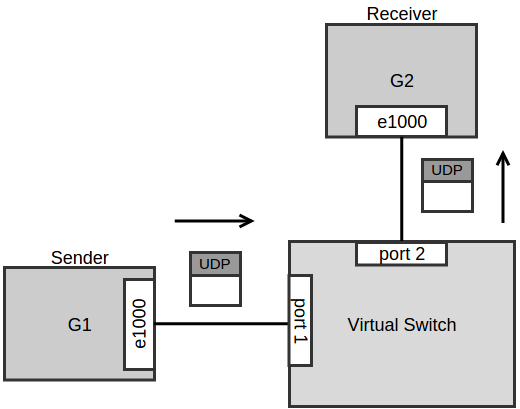
\includegraphics[scale=0.5]{img/g2g_comm.png}
	\caption{An UDP sender running on G1 sends packets to an UDP receiver running on G2. The VMs can communicate with each other through a virtual switch.}
	\label{img:g2g_comm}
\end{figure}
\section{Analysis of current implementation}
Now we are going to discuss about the performance of the current implementation (see section~\ref{sec:e1000_emu}~\footnote{For now we keep both TX and RX descriptor caches enabled.}) using both host-only and netmap networking modes.
\\
\\
In this section we will make two experiments, both with G1 acting as a sender and G2 acting as a receiver. In the first experiment we will run a simple application that will send (receive) UDP packets using a simple UDP socket in an infinite loop. This will be our first reference in terms of performance. In the second experiment, instead, we will run the aforementioned pkt-gen application that will make use of the netmap framework. This application is just an infinite loop that, for each iteration, fills its local netmap TX ring with a batch of packet (256) and performs a TX operation. In both cases, the packets are 60 bytes long.
%\begin{figure}[!h]
%	\centering
%	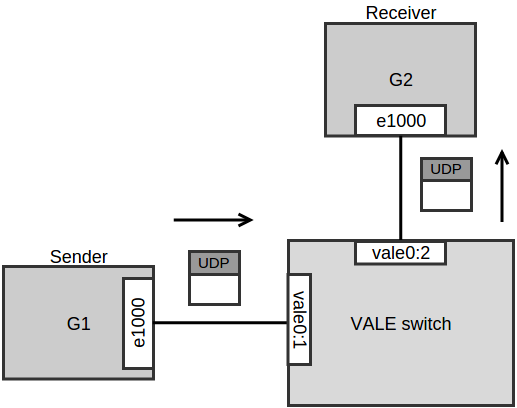
\includegraphics[scale=0.5]{img/G2G_netmap.png}
%	\caption{Type 2 System Virtual Machine generic architecture}
%	\label{img:g2g_netmap}
%\end{figure}
\subsection{Using host-only networking mode}
We first analyze the case where the VMs are connected with each other using the host-only networking mode, in particular using the \textit{vboxnet0} virtual switch provided by VirtualBox. We are going to analyze TX and RX performances separately.
\subsubsection{TX performance}
The measurements are shown in table~\ref{tab:vboxnet_tx}. All the values are computed counting the number of occurrences of each event over a period of 1 second and dividing the count itself for that time period.
\\
\\
When we use a UDP socket, we have a TX packet rate that is not really high, about 30.5 Kpps. We can see that there is a TX notification (i.e. TDT write) and an interrupt for each packet. \textit{TX descriptor load} is the number of times the emulation code accesses the guest physical memory to read the transmit descriptors, while \textit{TX descriptor fetched} is the average value of fetched TX descriptors in a single memory access.
\\
Even if we enabled the cache for transmit descriptors, we are not effectively taking advantage of it (only one fetched descriptor per memory access). This is due to the fact that we have one TX notifications per packet. When the device driver in the guest writes in the TDT register, the EMT performs a VM exit and executes the emulation code. As a result, when it wants to transmit, it finds only one descriptor that must be processed. After the descriptor processing, the EMT performs a VM entry and executes the device driver, that, in turn, will prepare another descriptor and write in TDT register and the EMT will go back to the emulation code in the host world. This procedure introduces a lot of overhead.
\\
\\
The problem of TX notification is not present when we run pkt-gen, since it exploits the modifications provided in the patched e1000 device driver. In fact, for each TXSYNC operation invoked by the application, the driver pushes down packets in batch, resulting in one TDT register write per batch instead of one TDT write per packet. As a result, we have an improvement of performance that is about 10 times than before (about 340 Kpps).

\begin{table}[t]
\centering
\begin{tabular*}{\textwidth}[tb]{l@{\extracolsep{\fill}}cc}
\toprule
\textbf{Measured quantity} & \textbf{UDP Socket} & \textbf{Netmap native mode}\\
\midrule
TX packet rate					&	30.5 KHz		&	340 Kpps\\\midrule
Interrupt rate					&	30.5 KHz		&	1.35 KHz\\\midrule
TX notifications					&	30.5 KHz		&	1.35 KHz\\\midrule
TX descriptors load				&	30.5 KHz		&	6.8 KHz\\\midrule
TX descriptor fetched (average)	&	1			&	51\\
\bottomrule
\end{tabular*}
\caption{This table shows statistics about the sender VM attached to the \textit{vboxnet0} virtual switch. The \textit{descriptor load} shows how many times the guest physical memory is accessed to read the TX descriptors.}
\label{tab:vboxnet_tx}
\end{table}

\subsubsection{RX performance}
All measurements are shown in table~\ref{tab:vboxnet_tx}. Again, the values are computed counting the number of occurrences of each event over a period of 1 second and dividing the count itself for that time period.
\\
\\
\begin{table}[t]
\centering
\begin{tabular*}{\textwidth}[tb]{l@{\extracolsep{\fill}}cc}
\toprule
\textbf{Measured quantity} & \textbf{UDP Socket} & \textbf{Netmap native mode}\\
\midrule
RX packet rate					&	30.5 Kpps	&	340 Kpps\\\midrule
Interrupt rate					&	14.8	 KHz		&	31.8 KHz\\\midrule
RX notifications					&	14.4 KHz	 	&	2.11 KHz\\\midrule
RX descriptors load				& 	2 KHz 		&	23.08 KHz\\\midrule
RX descriptor fetched (average)	&	15			&	15\\
\bottomrule
\end{tabular*}
\caption{This table shows some statistics about the receiver VM attached to the \textit{vboxnet0} virtual switch. In this case the RX descriptor cache is exploited.}
\label{tab:vboxnet_rx}
\end{table}When we use UDP Sockets the packet rate is the same as the transmitter, so it is able to receive all the packets coming from the switch. 
%Even if the receiver is able to receive all transmitted packets,  we can see a different interrupt rate. This means that the EMT on the receive side is slow. In this situation we have three threads that form a consumer-producer chain. This situation is depicted in figure~\ref{img:prod_cons}.
\\
We can see that the RX descriptor cache is exploited this time. This is due to the fact that the cached RX descriptors are the free descriptors that the adapter can fill with incoming packets (see section~\ref{subsec:rx_emulation}), so it is not strictly dependent on the RDT register writes performed by the device driver on the guest.
\\
\\
When we run pkt-gen, we can see an improvement of performance in terms of packet rate. In fact, we can see that the RX notification rate decreased greatly decreased even if the packet rate is about 10 time higher than the previous case. This is thanks to the fact that the modified e1000 driver writes to the RDT register only at the end of the interrupt routine, not for each packet. 
\\
We can also notice that the interrupt rate is much higher (31.8 KHz) with respect to the sender one (1.35 KHz). The reason is that, potentially, in the RX case an interrupt is raised for each received packet. This is unavoidable because the adapter cannot guess whether or not an incoming frame is the last of a batch.

%\begin{figure}[!t]
%	\centering
%	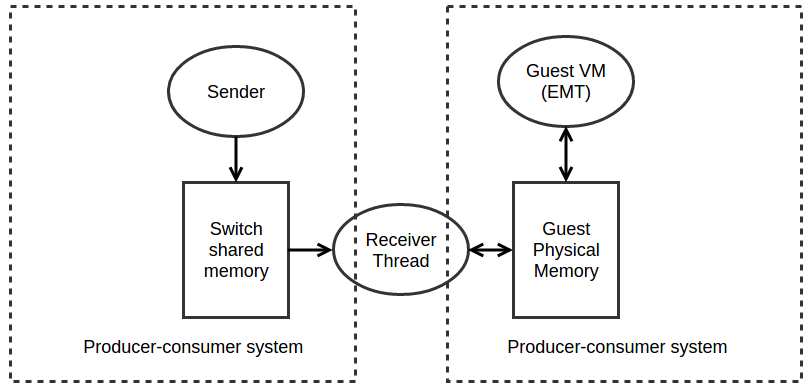
\includegraphics[scale=0.5]{img/prod-cons.png}
%	\caption{Two producer-consumer systems forming a chain. The first system is composed by the sender EMT as a producer and the Asynchronous I/O thread on the receive side as a consumer. The second system is composed by the the same asynchronous thread as a producer and the receiver EMT as a consumer.}
%	\label{img:prod_cons}
%\end{figure}
\subsection{Using netmap networking mode} \label{subsec:using_netmap_mode}
Now we analyze the case where the VMs are connected with each other using the netmap networking mode, in particular using the VALE virtual switch provided by netmap. 
\subsubsection{TX performance}
\begin{table}[t]
\centering
\begin{tabular*}{\textwidth}[tb]{l@{\extracolsep{\fill}}cc}
\toprule
\textbf{Measured quantity} & \textbf{UDP Socket} & \textbf{Netmap native mode}\\
\midrule
TX packet rate					&	23.8 Kpps	&	1.148 Mpps\\\midrule
Interrupt rate					&	23.8 KHz		&	3.8 KHz\\\midrule
TX notifications					&	23.8 KHz		&	4.5 KHz\\\midrule
TX descriptors load				&	23.8 KHz 	&	22.4 KHz\\\midrule
TX descriptor fetched (average)	&	1 			&	51\\\midrule
TXSYNC rate						&	26.3 KHz		&	1.148 MHz\\
\bottomrule
\end{tabular*}
\caption{This table shows some statistics about the sender VM attached to the \textit{vale0} virtual switch. In native mode we have a great improvement of performance in terms of packet rate.}
\label{tab:vale_tx}
\end{table}The measurements are shown in table~\ref{tab:vale_tx}.
\\
Using UDP packets, we have a packet rate that is even lower than the host-only case. This is due to the fact that, since the netmap connector is designed for packet batching, the overhead is not amortized over a batch of packets, so we have a decrease of performance.
\\
\\
In netmap native mode, instead, we can see that the performance dramatically increased to 1.148 Mpps, that is \textbf{over 3 times better} than the host-only case with the adapter in native mode.
\\
The TXSYNC rate shows how many times the TXSYNC operation is called in the connector. As we can see, we have one TXSYNC per frame. This means that, even if the e1000 adapter receives batches of packets, they are sent on the VALE switch one by one. Since the connector knows nothing about the packets arriving from the port, this situation is unavoidable, unless we do not modify the e1000 emulation code.
\\
Ultimately, if we were able to perform only one TXSYNC per batch, we would see a great improvement of performance. A solution will be presented in section~\ref{sec:packet_batching}.

\subsubsection{RX performance}
\begin{table}[t]
\centering
\begin{tabular*}{\textwidth}[tb]{l@{\extracolsep{\fill}}cc}
\toprule
\textbf{Measured quantity} & \textbf{UDP Sockets} & \textbf{Netmap native mode}\\
\midrule
RX packet rate					&	23.8 Kpps	&	588 Kpps\\\midrule
Interrupt rate					&	15 KHz		&	23.2 KHz\\\midrule
RX notifications					&	15 KHz		&	5.4 KHz\\\midrule
RX descriptors load				& 	1.7 KHz	 	&	42.7 KHz\\\midrule
RX descriptor fetched (average)	&	14 			&	14\\
\bottomrule
\end{tabular*}
\caption{This table shows some statistics about the receiver VM attached to the \textit{vale0} virtual switch. Also here, in native mode we have a great improvement of performance in terms of packet rate.}
\label{tab:vale_rx}
\end{table}The measurements are shown in table~\ref{tab:vale_rx}.
\\
As far as concerns UDP sockets experiment, all the discussions made for the previous cases are still valid.
\\
In netmap native mode, we can see a quite improvement of performance, about 3/4 times faster than the generic case, about 73\% than host-only case with the adapter in native mode. The reason why the performance are not as high as the transmission ones, resides in the interrupt rate. Since the adapter knows nothing about packet batches, it raises an interrupt as explained in section~\ref{subsec:e1000_interrupts}. Even if the connector is able to understand whether or not the current packet is the last one of the batches, there is no way to send this information to the port without modifying the port itself. Therefore, in order to improve performance, we must modify the e1000 emulation code. These modifications will be explained in section~\ref{sec:packet_batching}.

\section{Packet batching} \label{sec:packet_batching}
In the previous section we discussed about the performances using both host-only networking mode and and VALE switches, and we proved that we achieved very high performance using the latter.
\\
Moreover, we showed that we can further increase both TX and RX performances by making the connector and the port aware of packet batching. In this section we will present our solution.

\subsection{Implementation}
In order to achieve higher performance on both TX and RX sides, we made some  modifications on the e1000 port and on our netmap connector.

\subsubsection{TX path}
On the TX path, we modified both port and connector. In particular:
\begin{itemize}
\item We added some lines of code where the port calls the \textit{pfnSendBuf} callback on the connector. Before calling it, we check if the current outgoing frame is the last one in the batch by looking at TDT and TDH registers. 
\\
Let $N_s$ be the number of TX descriptors. If $$(TDT - TDH) \bmod N_s \equiv 1$$ then we set a flag (\textit{TXSYNC} flag) on the S/G data structure passed to the callback as an argument, so that the connector understands that this is the last frame in the batch.
\item In the implementation of the \textit{pfnSendBuf} callback in the connector, we check if the \textit{TXSYNC} flag is set. If this is the case, then we perform the TXSYNC operation, otherwise we just update the netmap indexes and return.
\end{itemize}
In that way, instead of doing a TXSYNC for each outgoing packet, we perform that operation only at the end of the batch.
\\
We must point out that we did not add anything new in the S/G data structure. In fact, this structure contains a string of 32 bits used for flags. 28 bits of this string are used for other purposes, while the remaining four bits are  available for new custom features.
\\
\\
The modification on the port has effect only in netmap networking mode, since the flag we set are checked only by our connector.

\subsubsection{RX path}
Also on the RX path, we modified both port and connector. In particular:
\begin{itemize}
\item In the asynchronous thread body, we enter a loop in which we call the \textit{pfnReceive} callback on the port until there are available incoming frames or until the port is not available for receiving anymore. After the loop, we added a further call to the \textit{pfnReceive} callback, passing a \textit{NULL} pointer instead of available data. This is our way to notify the port that there are no more packets in the batch.
\item We added a check on the \textit{pfnReceive} implementation of the e1000 port, in which we check the pointer to available data passed as argument. If it is \textit{NULL}, it means that the batch is finished, so we raise an interrupt and return.
\\
Moreover, since we want to raise an interrupt only in that case, we disabled all other interrupts in the receiving path. 
\end{itemize}
In this case the modifications we made are compatible \textbf{only} using the netmap networking mode and the e1000 device as emulated network adapter. In fact, the modified port will raise an interrupt \textbf{if and only if} it has a \textit{NULL} pointer as argument, but only our connector will pass this value to the port. Therefore, if we change the networking mode (e.g. host-only), the guest will not be able to receive any packets.
\\
The same \textit{may} happen if we change the port. Since it is not suppose to happen that a connector passes a \textit{NULL} value to the port instead of the available data, the effects of this particular function call may be unpredicted and may also cause a crash of the VM itself.

\subsection{Performance analysis}
\begin{table}[t]
\centering
\begin{tabular*}{\textwidth}[tb]{l@{\extracolsep{\fill}}cc}
\toprule
\textbf{Measured quantity} & \textbf{TX stats.} & \textbf{RX stats.}\\
\midrule
Packet rate							&	1.615 Mpps	&	940 Kpps\\\midrule
\textbf{Interrupt rate}				&	6.3 KHz		&	\textbf{2 KHz}\\\midrule
TX/RX notifications					&	6.3 KHz		&	83 KHz\\\midrule
Descriptors load						& 	32 KHz	 	&	63.2 KHz\\\midrule
Descriptor fetched (average)			&	51 			&	15\\\midrule
\textbf{TXSYNC}						&	\textbf{6.38 Khz}& /\\

\bottomrule
\end{tabular*}
\caption{This table shows statistics about both VMs attached to the \textit{vale0} virtual switch. We highlighted the items that caused the performances improvements.}
\label{tab:netmap_sync}
\end{table}
The results are shown in table~\ref{tab:netmap_sync}. As we can see, we have a great improvement of performances. We achieved 1.615 Mpps on the sender and  940 Kpps on the receiver.
\\
As highlighted in the table, we can see that the TXSYNCs are performed only at the end of the batch. Also the interrupt raised to the guest from the port are now amortized over the batch.
\\
\\
\begin{figure}[!t]
	\centering
	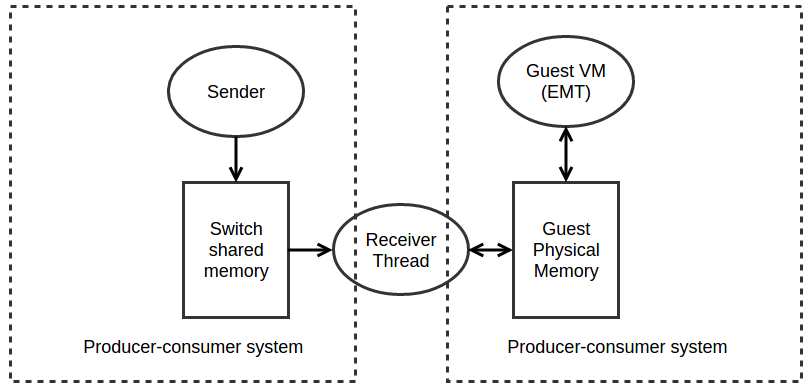
\includegraphics[scale=0.5]{img/prod-cons.png}
	\caption{Two producer-consumer systems forming a chain. The first system is composed by the sender EMT as a producer and the Asynchronous I/O thread on the receive side as a consumer. The second system is composed by the the same asynchronous thread as a producer and the receiver EMT as a consumer.}
	\label{img:prod_cons}
\end{figure}We can also notice that the receive rate is less than the transmit rate. That is caused by a bottleneck in a chained producer-consumer system.
\\
Figure~\ref{img:prod_cons} depicts our situation. We have the sender EMT that sends frame using the virtual switch. The receiver thread reads the new available data, writes them in the guest physical memory, and raises an interrupt to the guest so that the EMT of the receiver VM can consume the new data.
\\
In this system, the slow part is on the receive side. The reasons for this slowness are multiple, such as synchronization between the receiver thread and the receiver EMT and context switches between guest world and host world. The overhead introduced by these factors is not manageable since it is strictly dependent on the computation power of the host.

\section{Implementing mapping of descriptors} \label{subsec:memmap}
Looking at the previous tables, in particular table~\ref{tab:netmap_sync}, we can see the \textit{Descriptor load} row, which has a value of 32 KHz for transmitter and 63.2 KHz for receiver. As already mentioned, this value measures the accesses in guest physical memory performed by the emulated adapter. Each guest physical memory access involves an address translation, that implies some overhead. At \textit{normal} packet rates (e.g. about 30 Kpps), this overhead is negligible, but when we deal with very high packet rates, this becomes notable.
\\
Therefore, we adopted a solution that avoids those translations by \textit{mapping} a portion of the \textbf{guest physical} memory into the \textbf{host virtual} memory, so that the descriptors can be accessed by the host world using pointers.
\subsection{Memory region containing descriptors}
In order to map the e1000 descriptors in the host virtual memory, we need to know where the descriptors are located in the guest physical memory. To do so, we look at the aforementioned \textit{TDBAH} and \textit{TDBAL} registers for TX descriptors, and \textit{RDBAH} and \textit{RDBAL} registers for RX descriptors. In this way, we find the base address of the physical pages containing the descriptors.
\\
Moreover, the \textit{TDLEN} and \textit{RDLEN} registers contain the length in bytes of the physical memory occupied by the TX descriptors and RX descriptors, respectively. 
\\\\
\begin{figure}[!t]
	\centering
	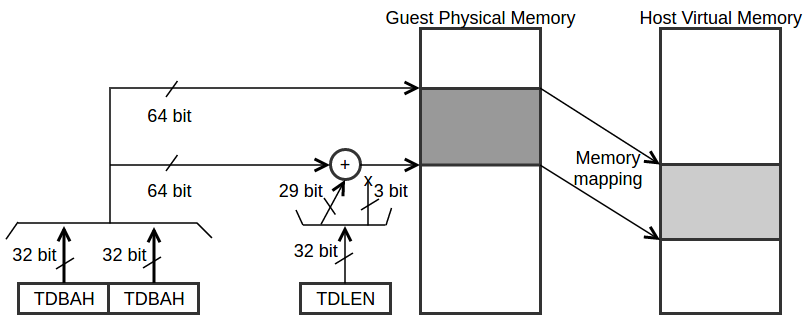
\includegraphics[width=\textwidth]{img/phys_mem.png}
	\caption{The mapped memory region for TX descriptors. The RX descriptor are mapped in the same way, but with the RX related registers. Notice that TDLEN is right-shifted by 3. This represent the division by 8.}
	\label{img:memmap}
\end{figure}Since the descriptors must be accessed in DMA by the adapter, we have the guarantee that the descriptors are allocated in contiguous pages~\footnote{In most Operating Systems, the size of a page is 4 Kilobytes.} in physical memory.
\\
Therefore, the mapped region will start from the base address $$TDBAH|TDBAL$$ up to  $$TDBAH|TDBAL + TDLEN / 8$$ address for the TX descriptors~\footnote{The mapping of RX descriptors is analogous.}.
\\
Figure~\ref{img:memmap} depicts the memory region mapped in the host virtual memory.
\\
\\
Since each descriptor is 16 bytes long, and a memory page is 4 kilobytes, in a single page we can map up to 256 descriptors, which is the default number of descriptors per ring that the device driver sets by default.
Furthermore, the e1000 devices support up to 4096 descriptors per ring, so our implementation supports the mapping of up to 16 memory pages, containing 256 descriptor each.

\subsection{Implementation}
Since we want to map the descriptors, we do not need any descriptor cache. Therefore, we disabled both TX and RX descriptor caches on the e1000 emulation code.
\\
\\
We implemented the mapping of the region using a function provided by VirtualBox: \textit{PDMDevHlpPhysGCPhys2CCPtr}. This function maps a guest physical memory page into the virtual memory of the host. It takes, among the others, the base address of the physical memory and a pointer that, after the execution of the function, will be used to access the mapped page.
\\
Since the base address of the descriptors may change during the execution of the VM (i.e. the value TDBAH/RDBAH and TDBAL/RDBAL registers), or even the number of descriptors itself (i.e. TDLEN/RDLEN), we customized the callback functions for write operation of these registers so that we can remap the pages when the registers values change.
\\
The mapping function is only available in R3 context, but the callbacks are always called in R0 context. Therefore, we added two new event queues to the port, one for TX descriptors, one for RX descriptors (see section~\ref{sec:e1000_emu}). When there is a write in one of the descriptors-related registers, the EMT:
\begin{enumerate}
\item Stores the old value of the register.
\item Updates the register.
\item Since it is in R0 context, posts an item in the event queue, so that it will execute the related callback after it switches to R3 context, but before it resumes executing guest code.
\item Executes the related callback function. This function checks whether or not the new value is equal to the old value. If it is true, then simply returns, otherwise it unmaps all the mapped memory pages (if any) and remaps them back using the new value of the register.
\end{enumerate}
All these operations may be expensive in terms of execution time, but since a remapping operation seldom happens (e.g. the reset of the adapter), its cost is well amortized.
\\
\\
This new optimization is completely compatible with other networking modes, since it does not affect the interaction between port and connector.
\subsection{Performance analysis}
Thanks to this optimization, we do not need to translate the guest physical address each time we need a descriptor. Instead, we can directly access it by means of a pointer.
\\
Table~\ref{tab:netmap_mapping} shows the performances in both TX and RX sides.
\\
\\
We can see that we have an improvement of performance in terms of packet rates that is 33\% in TX case and 45\% in RX case.
\\
Since we disabled descriptors caches, the adapter would have loaded only one descriptor per memory access. Therefore, thanks to memory mapping, we saved the overhead time that a total of \textbf{3.5 millions} of address translations would have caused for each packet. 
\begin{table}[t]
\centering
\begin{tabular*}{\textwidth}[tb]{l@{\extracolsep{\fill}}cc}
\toprule
\textbf{Measured quantity} & \textbf{TX stats.} & \textbf{RX stats.}\\
\midrule
Packet rate							&	2.2 Mpps		&	1.370 Mpps\\\midrule
Interrupt rate						&	8.9 KHz		&	2.8 KHz\\\midrule
Descriptors accesses					& 	2.2 MHz	 	&	1.37 MHz\\
\bottomrule
\end{tabular*}
\caption{This table shows the performances when we enable both packet batching and memory mapping. Since we disabled descriptors caches, we have an access for each packet transmitted/receive}
\label{tab:netmap_mapping}
\end{table}

\section{Code optimization}
We can further improve performance by means of small optimizations in the e1000 port.
\\
The emulation code contains some statements that are not useful (e.g. collecting statistics) and, at very high packet rates, introduce a notable overhead because they are executed for each single packet. We deleted those statements to improve performance:
\begin{itemize}
\item \textit{Useless lock acquisitions} Acquiring a lock may cause overhead. In the code there are some locks that are useless: as a matter of fact, also the documentation contained in the code itself says that one of these locks is useless. Therefore, we eliminated these locks.
\item \textit{Collecting statistics} In the code there are some functions whose purpose is to collect some statistics. These functions introduce overhead since they need to acquire a lock (that we already deleted) but also they perform some memory comparisons that introduce some overhead. Therefore, we deleted the calls to those functions.
\item \textit{Extra memory copy} In the RX path, for each received packet, there is copy from a local buffer to another local buffer, which is completely useless. Therefore, we avoid this extra copy.
\end{itemize}
As already mentioned, these statements would not affect performance with normal rates, but since we are dealing with millions of packets per second, the effect of a negligible overhead is amplified hundreds of times, so that it becomes notable.
\\
In table~\ref{tab:netmap_minors} the packet rates after these optimizations are shown.
\\
\\
As we can see, we have an improvement in terms of rate of received packets, while the TX packet rate remains equal to the previous case. This is due to the fact that the optimizations mostly concern the RX path, and, moreover, this is is the part that is strictly related to the computation power of the host. Therefore, it is easy to understand that avoiding statements that imply some expense in terms of computation time, it can quite improve performance.
\begin{table}[t]
\centering
\begin{tabular*}{\textwidth}[tb]{l@{\extracolsep{\fill}}cc}
\toprule
\textbf{Measured quantity} & \textbf{TX stats.} & \textbf{RX stats.}\\
\midrule
Packet rate							&	2.2 Mpps		&	1.750 Mpps\\
\bottomrule
\end{tabular*}
\caption{This table shows the packet rates after our code optimizations and when we enable both packet batching and memory mapping. We have an improvement only on RX side because it is the one that mostly depends on the computation power of the host.}
\label{tab:netmap_minors}
\end{table}

\chapter{Conclusions}
%\begin{table}[!h]
%\centering
%\begin{tabular*}{\textwidth}[tb]{l@{\extracolsep{\fill}}cc}
%\toprule
%\textbf{Measures} & \textbf{Host-only mode} & \textbf{Optimized netmap mode}\\
%\midrule
%TX Packet rate		&	340 Kpps		&	2.2 Mpps\\\midrule
%RX Packet rate		&	340 Kpps		&	1.75 Mpps\\
%\bottomrule
%\end{tabular*}
%\caption{This table shows the packet rates using host-only networking mode, netmap networking mode without optimizations and netmap networking mode with optimizations.}
%\label{tab:conclusion}
%\end{table}
In this work we showed the architecture of VirtualBox, in particular we gave details on the virtualization and networking architecture parts. We then presented our extension to VirtualBox so that it can support the netmap framework, implementing a new connector that is able to connect a VM to a VALE virtual switch. Subsequently, we analyzed the performance of the existing implementation using an e1000 device as virtual adapter and comparing the performances with the host-only networking mode and our new extension, pointing out the bottlenecks and problems. We also presented solutions to these problems exploiting packet batching, memory mapping and optimization of the e1000 emulation code in order to further improve performance.
\\
\\
We successfully improved performance starting from 340 Kpps in the host-only case, both TX and RX rates, achieving up to 2.2 Mpps in transmission and 1.75 Mpps in reception using netmap mode with optimizations. This means that we improved the TX packet rate of \textbf{6.5 times} and the RX packet rate of \textbf{5 times} with respect to host-only mode.

%\addcontentsline{toc}{section}{\refname}
\begin{thebibliography}{30}
\bibitem{netmap} \autori{Rizzo L.} \textit{netmap: a novel framework for fast packet I/O}
\bibitem{vbox} VirtualBox user manual. \url{https://www.virtualbox.org/manual/}
 \url{http://info.iet.unipi.it/~luigi/papers/20120503-netmap-atc12.pdf}
\bibitem{vale} \autori{Rizzo L., Lettieri G.} \textit{VALE: a switched ethernet for virtual machines.} \url{http://info.iet.unipi.it/~luigi/papers/20121026-vale.pdf}
\bibitem{amd-v} \autori{AMD} \textit{Secure Virtual Machine Architecture Reference Manual.}
\bibitem{vt-x} \autori{Neiger, Gil Santoni, A.} Intel virtualization technology: Hardware support for efficient processor virtualization. \textit{Intel Technology Journal 10, 3 (2006)}
\bibitem{iommu} \autori{Yehuda, B.} Utilizing IOMMUs for virtualization in linux and xen.
\bibitem{vmm_opt} \autori{Agensen, O., Mattson, J., Rugina, R., Sheldon, J.} Software techniques for avoiding hardware virtualization exits.
\bibitem{virtio} \autori{Russel, R.} virtio: towards a de-facto standard for virtual I/O devices.
\bibitem{rings} \autori{Intel} \textit{Intel 64 and IA-32 Architectures Software Developer's Manual}.
\bibitem{e1000} \autori{Intel} \textit{PCI/PCI-X Family of Gigabit Ethernet Controllers Software Developers Manual.}
\bibitem{sdl} SDL project. \url{http://www.libsdl.org/index.php}
\bibitem{qt} Qt project. \url{http://www.qt.io/}
\end{thebibliography}
	
\end{document}